\documentclass[11pt,a4paper]{report}

\usepackage[english]{babel} % Englisch und englische Rechtschreibung
\usepackage[utf8]{inputenc} % Unicode Text 
\usepackage[T1]{fontenc} % Umlaute und deutsches Trennen
\usepackage{textcomp} % Euro
\usepackage[hyphens]{url}
% statt immer Ab\-schluss\-ar\-beit zu schreiben
% einfach hier sammeln mit -. 
\hyphenation{Ab-schluss-ar-beit}
% Vorsicht bei Umlauten und Bindestrichen
\hyphenation{Ver-st\"ar-ker-aus-gang}
 % eigene Hyphenations, die für das Dokument gelten
\usepackage{amssymb} % Symbole
\usepackage{emptypage} % Wirklich leer bei leeren Seiten

%% Fonts, ein kompletter Satz an Optionen

% Times New Roman, gewohnter Font, ok tt und serifenlos
%\usepackage{mathptmx} 
%\usepackage[scaled=.95]{helvet}
%\usepackage{courier}

% Palatino mit guten Fonts für tt und serifenlos
\usepackage{mathpazo} % Palatino, mal was anderes
\usepackage[scaled=.95]{helvet}
\usepackage{courier}

% New Century Schoolbook sieht auch nett aus (macht auch tt und serifenlos)
%\usepackage{newcent}

% Oder default serifenlos mit Helvetica 
% ich kann es nicht mehr sehen ...
%\renewcommand{\familydefault}{\sfdefault}

\usepackage{microtype}

% Bilder und Listings
\usepackage{graphicx} % wir wollen Bilder einfügen
\usepackage{subfig} % Teilbilder
\usepackage{wrapfig} % vielleicht doch besser vermeiden
\usepackage{listings} % schöne Quellcode-Listings
% ein paar Einstellungen für akzeptable Listings
\lstset{basicstyle=\ttfamily, columns=[l]flexible, mathescape=true, showstringspaces=false, numbers=left, numberstyle=\tiny}
\lstset{language=python} % und nur schöne Programmiersprachen ;-)
% und eine eigene Umgebung für Listings
\usepackage{float}
\newfloat{listing}{htbp}{scl}[chapter]
\floatname{listing}{Listing}

% Seitenlayout
\usepackage[paper=a4paper,width=14cm,left=35mm,height=22cm]{geometry}
\usepackage{setspace}
\linespread{1.15}
\setlength{\parskip}{0.5em}
\setlength{\parindent}{0em} % im Deutschen Einrückung nicht üblich, leider

% Seitenmarkierungen 
\newcommand{\phv}{\fontfamily{phv}\fontseries{m}\fontsize{9}{11}\selectfont}
\usepackage{fancyhdr} % Schickere Header und Footer
\pagestyle{fancy}
\renewcommand{\chaptermark}[1]{\markboth{#1}{}}
%\fancyhead[L]{\phv \leftmark}
\fancyhead[L]{\phv \nouppercase{\leftmark}}
\fancyhead[R]{\phv \thepage}
% Unten besser auf alles Verzichten
%\fancyfoot[L]{\textsf{\small \kurztitel}}
\fancyfoot[C]{\ } % keine Seitenzahl unten
%\fancyfoot[R]{\textsf{\small Medieninformatik}}

% Theorem-Umgebungen
\newtheorem{definition}{Definition}[chapter]
\newtheorem{satz}{Satz}[chapter]
\newtheorem{lemma}[satz]{Lemma} % gleicher Zähler wie Satz
\newtheorem{theorem}{Theorem}[chapter]
\newenvironment{beweis}[1][Beweis]{\begin{trivlist}
\item[\hskip \labelsep {\textit{#1 }}]}{\end{trivlist}}
\newcommand{\qed}{\hfill \ensuremath{\square}}

% Quellen teilen
\usepackage{bibtopic} 

% Hochschule Logo, noch nicht perfekt
\usepackage{hsrmlogo}

% Spezialpakete
\usepackage{epigraph}
\setlength{\epigraphrule}{0pt} % kein Trennstrich

% damit wir nicht so viel tippen müssen, nur für Demo 
\usepackage{blindtext} 

% Zum Zeigen von Fehlern
\usepackage{soul}
\newcommand*\falsch{\st}



\usepackage{amsmath}
\usepackage{csquotes}
\usepackage{hyperref}
\usepackage{makecell}
\usepackage{multirow}
\usepackage{pgfplots}
\usepackage{siunitx}
\usepackage{tabularx}
\usepackage{xcolor}

\pgfplotscreateplotcyclelist{tb}{
    thick,tb_color_1 \\
    thick,tb_color_2 \\
    thick,tb_color_3 \\
    thick,tb_color_4 \\
    thick,tb_color_5 \\
    thick,tb_color_6 \\
    thick,tb_color_7 \\
}

\definecolor{tb_color_1}{HTML}{b71c1c}
\definecolor{tb_color_2}{HTML}{ff6f00}
\definecolor{tb_color_3}{HTML}{ffeb3b}
\definecolor{tb_color_4}{HTML}{212121}
\definecolor{tb_color_5}{HTML}{4caf50}
\definecolor{tb_color_6}{HTML}{2196f3}
\definecolor{tb_color_7}{HTML}{9c27b0}

\newcommand{\welchethesis}{Master}
\newcommand{\thesisofwas}{of Science}
\newcommand{\titel}{An Open-World Extension to Rule-Based Knowledge Graph Completion}
\newcommand{\autor}{Tobias Uhmann}
\newcommand{\datum}{17. Mai 2021}
\newcommand{\ort}{Wiesbaden}
\newcommand{\referent}{Prof.\ Dr.\ Adrian Ulges}
\newcommand{\korreferent}{Dr.\ Jörn Hees}

\begin{document}

    %
% Titelseite
%

\begin{titlepage}
    \begin{center}
    
    \hsrmlogo[1]
    \parbox[b]{8cm}{
        Hochschule RheinMain \\
        Fachbereich Design Informatik Medien \\
        Studiengang Informatik
    }
    
    \vfill
    
    {\LARGE Abschlussarbeit} \\[5mm]
    {\large zur Erlangung des akademischen Grades} \\[5mm]
    {\large \welchethesis\ \thesisofwas} \\[5mm]
    
    \rule{\textwidth}{1pt} \\[5mm]
    {\begin{spacing}{1.15} \huge \bfseries \titel \\ \end{spacing}}
    \rule{\textwidth}{1pt}
    
    \vfill
    
    \begin{tabular}{ll}
        Vorgelegt von & \autor       \\
        am            & \datum       \\
        Referent      & \referent    \\
        Korreferent   & \korreferent
    \end{tabular}  
    
    \vfill
    
    \end{center}
\end{titlepage}

\cleardoublepage

%
% Erklärung
%

\thispagestyle{empty}

% Erklärung gemäß den Allgemeinen Bestimmungen für Prüfungsordnungen
% der Paragraph schwankt, daher ohne Nennung einer Nummer
\section*{Erklärung gemäß ABPO}

Ich erkläre hiermit, dass ich
\begin{itemize}
    \item die vorliegende Abschlussarbeit selbstständig angefertigt,
    \item keine anderen als die angegebenen Quellen benutzt,
    \item die wörtlich oder dem Inhalt nach aus fremden Arbeiten entnommenen 
          Stellen, bildlichen Darstellungen und dergleichen als solche genau 
          kenntlich gemacht und
    \item keine unerlaubte fremde Hilfe in Anspruch genommen habe.
\end{itemize}

\vspace{6em}
\noindent\begin{tabular}{p{0.37\textwidth}p{0.56\textwidth}}
    \ort, \datum & \rule{0.56\textwidth}{0.5pt} \\
                 & \makebox[1cm]{\ } \autor
\end{tabular}

\vfill

\section*{Erklärung zur Verwendung der \welchethesis thesis}

Hiermit erkläre ich mein Einverständnis mit den im folgenden aufgeführten 
Verbreitungsformen dieser Abschlussarbeit:

\vspace{1em}
\noindent\begin{tabular}{|p{0.82\textwidth}|c|c|}
    \hline
    
    \textbf{Verbreitungsform} & 
    \makebox[0.035\textwidth]{\textbf{Ja}} & 
    \makebox[0.05\textwidth]{\textbf{Nein}} \\\hline
    
    Einstellung der Arbeit in die Hochschulbibliothek mit Datenträger & 
    $\times$ &
    \\\hline
    
    Einstellung der Arbeit in die Hochschulbibliothek ohne Datenträger & 
    $\times$ &
    \\\hline
    
    Veröffentlichung des Titels der Arbeit im Internet & 
    $\times$ &
    \\\hline
    
    Veröffentlichung der Arbeit im Internet & 
    $\times$ &
    \\\hline
\end{tabular}

\vspace{6em}

\noindent\begin{tabular}{p{0.37\textwidth}p{0.56\textwidth}}
    \ort, \datum & \rule{0.56\textwidth}{0.5pt} \\
                 & \makebox[1cm]{\ } \autor
\end{tabular}

\cleardoublepage


    \begin{abstract}

        Knowledge graphs store facts about objects in a graph structure. The graph's nodes represent entities while its edges represent relationships between the objects. Typical application scenarios include voice assistants and recommender systems. However, large knowledge graphs are usually incomplete and need to be updated continuously. AI approaches can support this task by suggesting probable facts that can be inferred from the existing graph.

        Most recent knowledge graph completion models approached the problem successfully by embedding the graph in a low-dimensional vector space. Further extensions to those embedding-based approaches make use of textual information to enable predictions about open-world entities for whom no facts are known in the existing graph. Alternative to embedding-based approaches, symbolic, rule-based systems capture patterns in the graph structure in form of logical rules. Recent works have shown that rule-based models can perform as well as embedding-based approaches and have the advantage that the model's rule-based decisions are comprehensible by humans.

        In this work, the Power model, an ensemble model consisting of a rule-based and a text-based KGC model is introduced. The rule-based component employs rules mined by the rule miner AnyBURL to make predictions based on the graph's structure, while the text-based component leverages additional text information about the entities to improve performance and enable prediction for open-world entities, which cannot be handled by the rule-based system. Furthermore, Power explains its predictions by giving the rules and text prioritization that led to its decision. The text prioritization is achieved by using an attention mechanism that focuses on those texts that are most relevant. The texts are encoded using contextual word embeddings produced by a variant of the state-of-the-art BERT transformer, which is shown to improve performance compared to the usage of conventional, static word embeddings. Finally, it is shown that the ensemble model produces better results than the rule- and text-based models on their own.

    \end{abstract}

    \setcounter{tocdepth}{4}
    \tableofcontents
    \newpage


    \chapter{Introduction}
    \label{ch:1_introduction}
    \emph{Knowledge graphs} (KGs) power search engines, question-answering systems, and social networks. They are especially useful to manage dynamic, diverse data and have drawn significant attention from industry and academia in recent years~\cite{}. Today, many big tech companies, such as Amazon~\cite{AmazonKG}, Facebook~\cite{}, Google~\cite{} and Microsoft~\cite{MicrosoftKG} run their own enterprise knowledge graphs. But, although the term ``Knowledge Graph'' became popular only in 2012 when Google announced its equally named system~\cite{}, the concept behind it is much older and even the term itself has been used back in the 70s~\cite{}.

Since then, many definitions for knowledge graphs have been given~\cite{}, often contradicting each other~\cite{}, but in general most describe knowledge graphs as directed graphs whose nodes and edges represent objects and their relationships to each other. In this work, a knowledge graph $G$ is formally defined as a set of known facts, which are a subset of all facts that could theoretically be constructed between the set of entities $E$ and the set of relations $R$:

\[
    G \subseteq E \times R \times E
\]

Due to their mathematical structure, facts are also referred to as \emph{triples}. A fact $(head, rel, tail)$ consists of a \emph{head} entity, a \emph{tail} entity and a relation between the two. Relations are usually not symmetrical and therefore represented by directed edges. \autoref{fig:1_introduction/knowledge_graph} shows an example knowledge graph as it could be used in a social network. It stores knowledge about concrete objects as well as general concepts, such as the fact $(Ed, has~gender, male)$. Symmetrical relations, such as ``married to'' are represented by two directed edges.

\begin{figure}[t]
    \centering
    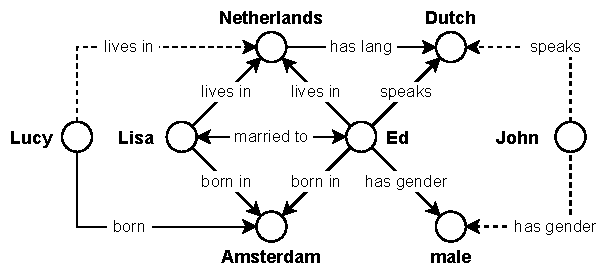
\includegraphics[]{1_introduction/knowledge_graph}
    \caption{Example Knowledge Graph. Nodes represent entities, while directed edges represent true facts consisting of the connected entities and a relation. Under the open-world assumption, the absence of facts does not necessarily mean they are false. Some missing, and yet true, facts are marked by dotted edges - they should be predicted by a KGC model.}
    \label{fig:1_introduction/knowledge_graph}
\end{figure}

Besides displaying known facts using solid lines, \autoref{fig:1_introduction/knowledge_graph} also shows dotted lines which indicate facts that hold true in reality but which are missing from the graph, like the fact $(Lucy, lives~in, Netherlands)$. Actually, real-world knowledge graphs are often rather incomplete for several reasons: First, it is difficult to manually create and update a large graph, and second, facts are sometimes deliberately left out if they can be derived from other facts. An example for the latter would be the transitive relation ``lies in'': Given a graph that stores $(Paris, lies~in, France)$ and $(France, lies~in Europe)$, it can be derived that Paris lies in Europe. This circumstance, that given facts can be relied on, but missing facts are not automatically false, but rather unknown, is known as \emph{open-world scenario}. In contrast to this is the \emph{closed-world assumption}, which states that non-existent facts are false.

When looking close at \autoref{fig:1_introduction/knowledge_graph}, patterns can be found in the graph structure. For example, two out of three people born in Amsterdam also speak Dutch. One could therefore correctly assume that this is also true for the third entity Lucy. Furthermore, the fact that person A is married to person B also seems to imply that person B is married to person A. Such patterns can be captured using two fundamentally different approaches, by (1) generalizing individual cases to logical \emph{rules} or by (2) \emph{embedding} the graph into a continuous vector space, which represents the patterns in a way that can be directly processed by machine learning models.

Many current state-of-the-art models follow the embedding approach, as it proved effective and efficient for a wide range of tasks including image~\cite{}, natural language~\cite{} and graph processing~\cite{}. Embedding-based approaches are also called \emph{latent}, because the exact structure of their embedding space is often incomprehensible, or latent, to humans. In contrast, classical rule-based approaches are denoted as \emph{symbolic} and bring the advantage that their rules are meaningful to humans -- other from a 300-dimensional vector in an embedding space. In their paper on the AnyBURL rule miner~\cite{}, Meilicke et al. show that rule-based models are capable to perform equally well to embedding-based approaches and demand further research on rule-based approaches.

Following that suggestion, this work builds a rule-based knowledge graph completion model on top of AnyBURL and combines it with a text-based model, forming the \emph{Power} ensemble model, which stands for ``\textbf{P}robabilistic \textbf{o}pen-\textbf{w}orld \textbf{e}xtension to \textbf{r}ule-based KGC''. Besides improving the rule-based model's fact predictions by leveraging additional text information, the text-based component enables predictions for open-world entities for which no facts are given. One of Power's top goals for both rule-based and text-based prediction is to explain its decision. Therefore, each predicted fact is given with a list of the rules and prioritization of the sentences that led to it.

As an example, considering the entity Lucy in \autoref{fig:1_introduction/knowledge_graph}, who is known to be born in Amsterdam, the Power model would suggest that she lives in the Netherlands and give the rule $(X, lives~in, Netherlands) <= (X, born~in, Amsterdam)$ with confidence of 67\% as an explanation. If multiple rules predict the same fact, all rules with a confidence greater 50\% are given in sorted order. In parallel to the rule-based prediction, a text about Lucy, like ``Lucy is from the Netherlands'', might lead to a 90\% prediction of $(Lucy, lives~in, Netherlands)$ by the text-based component. For open-world entities like John, the rule-based component cannot apply any rules, so analyzing John's texts is the only way to possibly predict his knowledge of Dutch or the fact that he is male. Again, multiple texts, like ``John is Dutch'' and ``He is an actor'', are sorted by relevance to explain to the user that the fact $(John, speaks, Dutch)$ was inferred due to the first sentence while the prediction of $(John, has~gender, male)$ is primarily based on the second one.

In the following, \autoref{ch:3_related_work} explains basics and terminology about neural networks and metrics that are used throughout this thesis. Next, \autoref{ch:2_basics} gives an overview of the variety of ways to approach knowledge graph completion using embedding and rule-based models before \autoref{ch:4_approach} explains the Power model's implementation. Subsequently, \autoref{ch:5_experiments} presents the evaluation results as well as experiments on variations of the Power model. \autoref{ch:6_conclusion} concludes with a summary and suggestions for further research. \autoref{ch:a_appendix} contains tables and graphs that have been separated for readability.

The Python implementation of the Power model is available on GitHub (\url{https://github.com/TobiasUhmann/power}) under the MIT open-source license. Additionally, multiple other repositories provide the code for the experiments~\cite{}.



    \chapter{Basics}
    \label{ch:2_basics}
    \section{Knowledge Graphs}
\label{sec:3_basics/1_knowledge_graphs}
One of the most popular knowledge graphs is Freebase~\cite{Bollacker2008FreebaseAC}. Although it is not maintained anymore since it was integrated into Wikidata in 2015~\cite{Tanon2016FromFT}, the benchmark datasets derived from it are still widely used. One of those benchmark datasets is the \emph{FB15k} dataset introduced by Bordes et al. in 2013~\cite{Bordes2013TranslatingEF}, which covers roughly \num{15000} Freebase entities. On its basis, Toutanova and Chen introduced the FB15k-237 subset in 2015~\cite{Toutanova2015ObservedVL}, whose purpose was to create a more meaningful benchmark by eliminating trivially predictable facts. For example, if FB15k-237 covers a relation like $(x, contains, y)$, it does not include its inverse relation $(y, part~of, x)$, because good performance resulting from such trivial, mutual predictions detracts from more interesting cases. In 2020, Safavi and Koutra published another dataset called CoDEx~\cite{Safavi2020CoDExAC}, which is derived from FB15k-237 and two other datasets, covers more diverse content and in turn poses a greater challenge than FB15k and FB15k-237. From the three provided variants of the CoDEx dataset -- CoDEx-S, CoDEx-M, and CoDEx-L -- the IRT approach by Hamann, on which this work is based, focuses on the CoDEx-M dataset. \autoref{tab:5_experiments/1_data_sources/1_knowledge_graphs/benchmark_datasets} gives an overview of the scales of FB15k, FB15k-237 and CoDEx-M. CoDEx-M actually contains additional, negative facts that are excluded here as this work focuses on the common open-world scenario.

\begin{table}[h]
    \centering
    \begin{tabular}{| l | r | r | r | r | r |}
    \hline

    \multicolumn{1}{|c|}{\textbf{Dataset}} &
    \multicolumn{1}{|c|}{\textbf{#Entities}} &
    \multicolumn{1}{|c|}{\textbf{#Relations}} &
    \multicolumn{3}{|c|}{\textbf{#Facts}} \\

    \multicolumn{1}{|c|}{} &
    \multicolumn{1}{|c|}{} &
    \multicolumn{1}{|c|}{} &
    \multicolumn{1}{|c|}{\textbf{Train}} &
    \multicolumn{1}{|c|}{\textbf{Valid}} &
    \multicolumn{1}{|c|}{\textbf{Test}} \\

    \hline \hline

    FB15k     & \num{14951} & \num{1345} & \num{483142} & \num{50000} & \num{59071} \\
    FB15k-237 & \num{14541} & \num{237}  & \num{272115} & \num{17535} & \num{20466} \\
    CoDEx-M   & \num{17050} & \num{51}   & \num{185584} & \num{10310} & \num{10311} \\

    \hline
\end{tabular}

    \caption{Comparison of popular KGC benchmark datasets}
    \label{tab:5_experiments/1_data_sources/1_knowledge_graphs/benchmark_datasets}
\end{table}

As for the above KGC benchmark datasets, a graph's fact set is usually further split into training, validation, and test subsets. Thereby, the splits are created so that there are training, validation, and test facts for possibly every entity. In contrast to that common approach, in his work on zero-shot learning, Hamann creates new \emph{IRT splits} from FB15k-237 and CoDEx-M that distinguish between so-called \emph{closed-world (CW) entities}, that are seen during training, and \emph{open-world (OW) entities}, which are not seen during training, to optimize prediction for unknown entities.

\begin{figure}
    \centering
    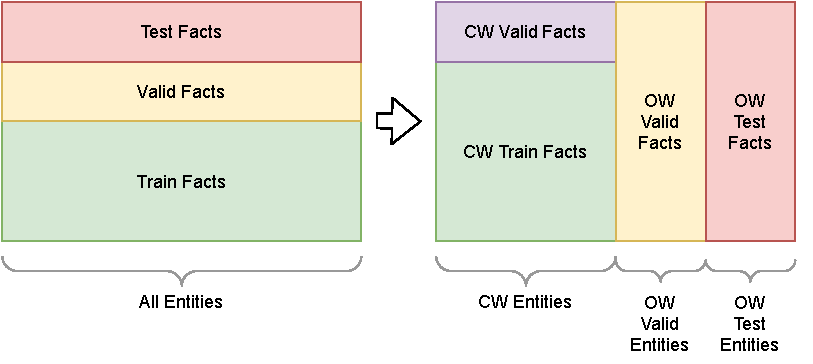
\includegraphics[width=\textwidth]{5_experiments/1_data_sources/1_knowledge_graphs/irt_split}
    \caption{Difference between a conventional and an IRT fact split. The IRT fact split focuses on open-world entities that must stay unseen during training. ``CW'' = ``closed-world'', ``OW'' = ``open-world''.}
    \label{fig:5_experiments/1_data_sources/1_knowledge_graphs/irt_split}
\end{figure}

\autoref{fig:5_experiments/1_data_sources/1_knowledge_graphs/irt_split} illustrates the different shape of an IRT fact split compared to a conventional one: The closed-world entities' facts are split into closed-world training and closed-world validation facts to enable closed-world prediction. Meanwhile, the open-world entities' facts are completely reserved for validation and training, respectively. Closed-world training and closed-world validation facts only refer to closed-world entities. On the other hand, one of an open-world validation fact's head or tail may also be a closed-world entity, and one of an open-world test fact's head or tail may be a closed-world entity or an open-world validation entity. \autoref{tab:5_experiments/1_data_sources/1_knowledge_graphs/irt_splits} gives an overview of the scales of the IRT splits' entity and fact subsets.

\begin{table}[h]
    \centering
    \begin{tabular}{ l c r r r c r r c r r }
    \toprule
    
    \multicolumn{1}{l}{\textbf{Graph}} & \phantom &
    \multicolumn{1}{c}{\textbf{\thead{CW \\ Train \\ Ents}}} &
    \multicolumn{1}{c}{\textbf{\thead{CW \\ Train \\ Facts}}} &
    \multicolumn{1}{c}{\textbf{\thead{CW \\ Valid \\ Facts}}} & \phantom &
    \multicolumn{1}{c}{\textbf{\thead{OW \\ Valid \\ Ents}}} &
    \multicolumn{1}{c}{\textbf{\thead{OW \\ Valid \\ Facts}}} & \phantom &
    \multicolumn{1}{c}{\textbf{\thead{OW \\ Test \\ Ents}}} &
    \multicolumn{1}{c}{\textbf{\thead{OW \\ Test \\ Facts}}} \\

    \midrule

    FB15k-237 && \num{12057} & \num{214412} & \num{23778} && \num{1545} & \num{46503} && \num{816}  & \num{25423} \\
    CoDEx-M   && \num{11399} & \num{123650} & \num{13738} && \num{2918} & \num{41240} && \num{1896} & \num{27577} \\

    \bottomrule
\end{tabular}

    \caption{Scale of the IRT splits of the FB15k-237 and CoDEx-M datasets}
    \label{tab:5_experiments/1_data_sources/1_knowledge_graphs/irt_splits}
\end{table}



\section{Rules}
\label{sec:3_basics/2_rules}
the facts in a KG are not random, can detect patterns
patterns can be described with first order logic, e.g. if a-r-b and a-r-c then a-r-d, or e.g. if a-r-b and a-r-c then a-r-d
in practice restrict to horn rules, humanly understandable and computational efficient (?)
example horn rule:

<example horn rule>

consists of rule body and head
body consists of one or more atoms.
atoms resemble facts, but head and tail can be variable

rule mining = find rules

\subsection{Rule Types}
\label{subsec:2_basics/2_rules/1_rule_types}
different types of rules can be found by different rule miners
e.g. cyclic/acyclic []

cyclic means ..

<example cyclic rule>

example for acylic:

<example acyclic rule>


\subsection{Rule Types}
\label{subsec:2_basics/2_rules/2_rule_metrics}
support, confidence, (lift)




\section{Neural Networks}
\label{sec:3_basics/3_neural_networks}
\emph{Neural networks} are a kind of machine learning models that are capable of detecting complex patterns in data. They consist of several \emph{layers} of connected \emph{neurons} that map input floating point vectors to output vectors. Figure~\ref{fig:2_basics/3_neural_networks/nn} shows an example of a neural network consisting of an input layer and two neural layers, also called \emph{linear layers}. The network forwards the input values on the left through the layers to produce the output values on the right.

\begin{figure}[t]
    \centering
    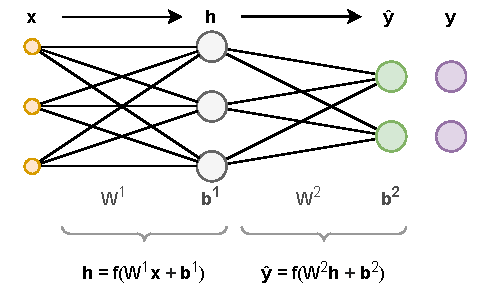
\includegraphics{2_basics/3_neural_networks/nn}
    \caption{Neural network consisting of the input layer, one hidden layer, and the output layer. The network's $l$th neural layer can be implemented by multiplying the layer's weight matrix $W^l$ with the layer input, adding the bias vector $b^l$, and applying the non-linear activation function $f$. By forwarding the network input $x$ through all layers, the network's output $\hat{y}$ is calculated as an approximation to the ground truth output $y$.}
    \label{fig:2_basics/3_neural_networks/nn}
\end{figure}

The values of each layer's output neurons are calculated as weighted sums of the input values. Subsequently, a constant \emph{bias} is added and a non-linear \emph{activation function} is applied. Graphically, the weights can be represented as edges between the input and output neurons, while the bias values are assigned to the output neurons. Mathematically, the function of a linear layer can be calculated using matrix multiplication. For a neural layer that maps a $d$-dimensional input vector to an $e$-dimensional output vector, the layer's weights can be represented by a $d \times e$ \emph{weight matrix}. The layer's output vector can then be calculated by multiplying the input vector with the weight matrix, adding the $e$-dimensional bias vector, and applying the activation function.

By cleverly combining linear layers, complex models can be created that vary the number of layers, the number of neurons per layer and the way neurons are connecte. During the last decade, exponentially increasing data and processing power made \emph{deep networks} consisting of many layers possible that have the advantage that they can work without sophistically encoded input data, because they come up with an encoding themselves. Other architecture concepts include \emph{recurrent neural networks (RNNs)}, that repeat certain layers multiple times and \emph{convolutional neural networks (CNNs)} that use filters to focus on local, close-by neurons. The semantics of the output layer's values depend on the network's intended task. An image \emph{classifier}, for example, yields probabilities that specify what output class the input most probably belongs to, while a \emph{natural language processing (NLP)} model might produce an abstract encoding of an input text.

To enable processing of the input data according to the desired output semantics, the parameters of the network, in particular the edge weights and bias vectors, need to have appropriate values. Which exact values are appropriate depends on the kind of input data, the network architecture, and the intended outputs. The optimal \emph{parameters}, to which the weights and biases count, are determined by \emph{training}, during which the network is repeatedly asked to make predictions for input data, which are then compared to the intended output data, the so-called \emph{ground truth}. In each step, the model's parameters are updated a bit to close the gap between predictions and ground truth. Specifically, the \emph{backpropagation} algorithm is used to calculate the gradient of a \emph{loss function} that quantifies the deviation between prediction and ground truth, and applies that gradient to the model's parameters layer by layer, starting with the output layer, thus backpropagating the change through the network. Formally, the models parameters $\theta$ at step $t+1$ are calculated as described in Equation~\ref{eq:2_basics/3_neural_networks/backprop}: The gradient of the loss function $L$ is multiplied by a \emph{learning rate} $\lambda$ and subtracted from the old parameter value.

\begin{align}
    \theta^{t+1} = \theta^t - \lambda \frac{\partial L(y, \hat{y})}{\partial \theta}
    \label{eq:2_basics/3_neural_networks/backprop}
\end{align}

In practice, the so-called \emph{optimizer} for calculating the parameter deltas from the gradient and applying them. The choice of the learning rate has a great influence on training: If the learning rate is too low, the training takes too long, but if it is too high, it can happen that the parameters are updated too much and cannot settle at their optimum. Furthermore, local minima and plateaus in the loss function make it hard to reach parameters that minimize the loss function most. Advanced optimizers therefore resort to techniques like momentum, where the previous learning progress is taken into account, or changing the learning rate over time to reach optimal parameters in a reasonable time. Furthermore, the choice of the loss function also has a significant influence on the learning success. The simple \emph{mean squared error (MSE)} loss serves its purpose, but advanced loss functions such as the \emph{binary cross entropy (BCE)} loss used for binary classification accelerate training significantly. Equations~\ref{eq:2_basics/3_neural_networks/mse} and~\ref{eq:2_basics/3_neural_networks/bce} compare the calculation of the MSE and BCE loss for a classifier with $n$ binary output classes.

\begin{align}
    L_{MSE}(y, \hat{y}) &= \frac{1}{n} \sum_{i=1}^n (y_i - \hat{y}_i)^2
    \label{eq:2_basics/3_neural_networks/mse} \\
    L_{BCE}(y, \hat{y}) &= \frac{1}{n} \sum_{i=1}^n y_i \cdot log( \hat{y}_i) + (1-y_i) \cdot log(1 - \hat{y}_i)
    \label{eq:2_basics/3_neural_networks/bce}
\end{align}

Besides selecting the appropriate learning rate, optimizer and loss function, it is important to avoid overfitting during training. This occurs when the model is trained for too long and the parameters are perfectly matched to the data used for training, but no longer work well on new data - in that case the model has learned the data by heart, so to speak. To prevent overfitting and identify the optimal time to stop training, the model is trained and validated on separate datasets. During training on the \emph{training data}, it is regularly checked how the model behaves on the unseen \emph{validation data}, whose loss eventually reaches a minimum and increases again, which serves as a sign to terminate training. In addition to training and validation data, a portion of the data, the \emph{test data}, is kept under lock until the final \emph{evaluation} of the model. The reason for this is that researchers use the validation results to optimize the model, in a sense hand-tailoring it to the validation data. Therefore, the test data may be evaluated only after all the optimizations of the model have been completed to provide an objective measure of generalization to unseen data.

As mentioned, neural networks proved successful in various domains, including NLP. Processing natural language opens many possiblities, for example, seamless human-machine interaction and knowledge extraction. What all NLP approaches have in common, is that they have to represent text in a way that makes it easy to process. The classical way to numericalize a text is using a \emph{bag of words}, which is a large vector whose elements represent words of a vocabulary. A concrete text is then encoded by setting all those elements to 1 that represent words occurring in the sentence. Allthough, the order of words is not preserved that way, bag of words have been used successfully with different machine learning models. A classical example would be a spam filter, implemented as a Bayesian network.

During the last decade, however, neural networks have had a breakthrough in NLP, because they solve a big problem of existing text encodings: Bag-of-words bear the problem that they are very \emph{sparse}, i.e. most entries are empty. Meanwhile,\emph{manually engineered feature vectors} that target this problem are not only time consuming to create, but often tailored for specific data. Since then, deep networks have arised and offer the ability to learn feature representations on their own - given enough time and training data. Due to the exponential growth in processing power and data, both constraints have been overcome, so that most state-of-the-art NLP models represent text using low-dimensional vectors, called \emph{embeddings}, today. They are called embeddings, because the low-dimensional vector space the words are projected into is very dense compared to previous sparse encodings, so one can image how words have to embedded into such an \emph{embedding space}. Thereby, low-dimensional typically refers to 50--300 dimensions.

Another breakthrough has been achieved in 2017 when \emph{transformers} outperformed other language models by far. Similar to the basic principle behind CNNs, transformers focus on those parts of the input data that are particularly important for current processing. The concept is referred to as \emph{attention}, because the transformer attends to certain words in its input text. Recently, the concept has also been applied to other domains, such as video processing, for example~\cite{Bertasius2021IsSA}. One drawback of transformers is their sheer size. For example, recently, Google has trained the first transformer with over a trillion parameters~\cite{Fedus2021SwitchTS} on the Colossal Clean Crawled Corpus - a text dataset of 800GB size in its default English version and of 26TB size in its multi-lingual version~\cite{C4}. As training such a large models takes very long, even when using specialized processors, researchers provide \emph{pre-trained} word embeddings that were obtained from training a large model on a general-purpose task, such as predicting missing words in gap texts, using common text data. Users can then take these pre-trained embeddings as a basis and \emph{fine-tune} them in regard to their specialized \emph{downstream task}.



\section{Metrics}
\label{sec:3_basics/4_metrics}
When designing and implementing machine learning models, scientists act on experience when it comes to architectural decisions and hyperparameter choices. In the early stages of a model, a trained eye on processing examples and observing the loss curve enable rapid progress. However, as the model matures, it becomes essential to quantify its performance with respect to comprehensive validation and test sets. Besides the selection of appropriate validation and test data, it is important to choose a meaningful metric that fits the problem. For example, when all of a models predictions are equally relevant, one would aim for an overall high precision, whereas a use case that involves a human processing the results manually, such as a web search, for example, one would choose a ranking metric that rewards good results at the top of a list.

All considered metrics are defined by terms from the so-called confusion matrix shown in Figure~\ref{fig:2_basics/4_metrics/1_confusion_matrix}. The matrix applies to the general scenario in which predictions are made about a certain condition for a set of objects. Thereby, an object's actual condition can be positive or negative, also referred to as its \emph{ground truth}, as can be the object's predicted condition. A prediction is \emph{true}, or correct, if its predicted condition is consistent with the object's actual condition and \emph{false} otherwise. Furthermore, objects whose prediction is positive are called \emph{positives}, while objects whose predictions are negative are called \emph{negatives}. Depending on their actual and their predicted condition, each object falls into one of four distinct categories:

\begin{figure}[t]
    \centering
    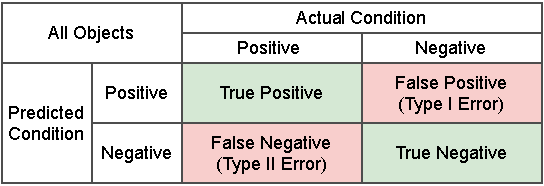
\includegraphics[width=\textwidth]{2_basics/4_metrics/confusion_matrix}
    \caption{Confusion Matrix dividing objects into four distinctive groups depending on their actual and predicted condition}
    \label{fig:2_basics/4_metrics/1_confusion_matrix}
\end{figure}

\begin{itemize}
    \item \textbf{\emph{True positives}} (TP) are objects for which the regarded condition is positive and whose predicted conditions is also positive.

    \item \textbf{\emph{False positives}} (FP) are objects for which the regarded condition is positive but whose predicted condition is negative. This type of error is referred to as a \emph{Type I error}.

    \item \textbf{\emph{False negatives}} (FN) are objects for which the condition is actually negative but whose predicted condition is positive. This second kind of errornous prediction is also referred to as \emph{Type II error}.

    \item \textbf{\emph{True negatives}} (TN) are objects for which the condition is actually negative and whose predicted condition is also negative.
\end{itemize}

Although it is generally desirable to obtain as many correct predictions as possible, true positives and true negatives are often differently important and errors of type one and two differently severe. In medicine, for example, not recognizing a disease could be much worse than accidentally diagnosing a healthy person as ill. Conversely, not recognizing guilt in a lawsuit might be less serious than convicting someone who is innocent. In the context of knowledge graph completion under the open-world assumption, the focus lies on true positives since the KGC model cannot make any qualified statements about false facts without negative samples in the graph. Omitting a fact from the prediction only means that the model has too little evidence for that fact, not that it can falsify it.

%The purpose of this section is to explain those metrics relevant for this work. Section~\ref{fig:2_basics/4_metrics/1_confusion_matrix} defines basic terms used by the following sections. Sections~\ref{subsec:2_basics/4_metrics/2_accuracy} and~\ref{subsec:2_basics/4_metrics/3_prf} then present the general purpose metrics accuracy, precision, recall and F1 score while Sections~\ref{subsec:2_basics/4_metrics/4_mrr} and~\ref{subsec:2_basics/4_metrics/5_map} discuss the ranking metrics MRR and mAP\@.

%\subsection{Confusion Matrix}
%\label{subsec:2_basics/4_metrics/1_confusion_matrix}
%All considered metrics are defined with the help of terms from a so-called confusion matrix as shown in Figure~\ref{fig:3_basics/4_metrics/1_confusion_matrix}. The matrix emerges from the general scenario in which predictions are made for a set of objects that can be either true or false. A prediction is true if its statement is consistent with reality about the object, also called ground truth, and false if the prediction contradicts reality. An example scenario would be an image recognition that has to determine whether a photo shows a cat or not. Then, four mutually exclusive types of predictions can be distinguished:

\begin{itemize}
    \item \textbf{\emph{True positives}} (TP) are predictions stating that a condition holds true when this is indeed the case. In the image recognition example, this would correspond to the case where the model correctly classifies a cat image as a cat.

    \item \textbf{\emph{False positives}} (FP) are negative predictions about objects where the condition is actually true, e.g. declaring an animal as cat although it is not. This type of error is also referred to as a \emph{Type 1 error}.

    \item \textbf{\emph{False negatives}} (FN) are another kind of erroneous predictions, also referred to as \emph{Type 2 errors}. They represent the case that an element with a true condition was classified as false - was overlooked, so to speak. An example would be a cat image not recognized as a cat.

    \item \textbf{\emph{True negatives}} (TN) are similar to true positives in that they are correct predictions, as well. They consist of rejective predictions about objects where the condition does indeed not apply, for example by recognizing that there is no cat in a cat-less photo.
\end{itemize}

Although it is generally desirable to obtain as many correct predictions as possible, true positives and negates are often differently important and errors of type one and two differently severe. In medicine, for example, not recognizing a disease could be much worse than accidentally diagnosing a healthy person as ill. Conversely, not recognizing guilt in a lawsuit might be less serious than convicting someone who is innocent. In the context of knowledge graph completion under the open-world assumption, the focus lies on true positives since the KGC model cannot make any qualified statements about non-applying facts without negative samples in the graph. Omitting a fact from the prediction only means that the model has too little evidence for that fact, not that it can falsify it.

\begin{figure}[t]
    \centering
    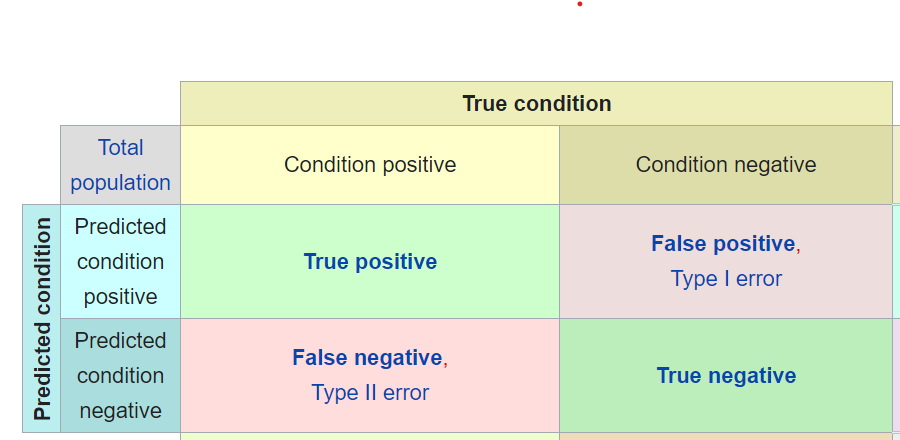
\includegraphics[width=\textwidth]{3_basics/4_metrics/1_confusion_matrix/matrix}
    \caption{Confusion Matrix}
    \label{fig:3_basics/4_metrics/1_confusion_matrix}
\end{figure}

"positive", "negative", "true", "false" predictions, "positive", "negative" elements

cat example
ir scenario


\subsection{Accuracy}
\label{subsec:2_basics/4_metrics/2_accuracy}
One of the most common general-purpose metrics is \emph{accuracy}, which measures a model's overall capability to make correct positive and negative predictions. In the case of binary classification, accuracy is the rate of correct predictions over all predictions:

\begin{align}
    Accuracy = \frac{TP + TN}{TP + TN + FP + FN}
    \label{eq:2_basics/2_metrics/1_accuracy/accuracy}
\end{align}

Colloquially speaking, accuracy answers the question of how good predictions are in general. It takes values in $[0, 1]$, whereby higher is better. However, although accuracy is a useful and intuitive metric in general, it can be misleading when it comes to unbalanced classes because a model can simply reach high accuracy by always predicting the predominant class. For example, if nine out of ten ground truth values are false, a model could reach 90\% accuracy by always predicting false. To counteract this, balanced accuracy~\cite{Mower2005PREPMtPR} can be used instead. However, as mention earlier, as negative predictions do not play a big role for KGC models in an open-world scenario, accuracy will only play a minor role in this work.


\subsection{Precision, Recall and F1}
\label{subsec:2_basics/4_metrics/3_prf}
\emph{Precision}, \emph{recall} and \emph{F1} focus on positive predictions. Precision gives an impression of how reliable positive predictions are, recall tells how many of the actual positive elements are declared as such, and F1 is a measure that combines both precision and recall in one value. All three metrics take values from $[0, 1]$ whereby higher is better.

Precision, also known as \emph{positive predictive value (PPV)}, is the ratio of true positive predictions to all positive predictions as noted in \autoref{eq:2_basics/2_metrics/2_prf/precision}. False negatives are not considered. If a model does not produce any predictions, precision is undefined and has to be defined in accordance with the evaluation scenario. One possibility is to define as 1 if the dataset does not contain any ground truth positives and 0 otherwise, because the model should not produce any predictions if, and only if, there are no ground truth positives.

\begin{align}
    Precision = \frac{TP}{TP + FP}
    \label{eq:2_basics/2_metrics/2_prf/precision}
\end{align}

Recall, on the other hand, also known as \emph{true positive rate (TPR)}, compares the number of true positives to the number of all ground truth positives as shown in \autoref{eq:2_basics/2_metrics/2_prf/recall}. False positives do not count in. If the evaluated dataset does not contain any ground truth positives, recall is undefined and might be specified as 1, because the model did not miss out on any ground truth positives.

\begin{align}
    Recall = \frac{TP}{TP + FN}
    \label{eq:2_basics/2_metrics/2_prf/recall}
\end{align}

Precision and recall are directly dependent on each other. A cautious model that only predicts positives when it is sure achieves high precision but low recall. Conversely, it is easy to achieve optimal recall by making positive predictions for all elements, though precision will suffer in that case. The \emph{F score} serves as a measure that considers both goals and reaches a high value when a reasonable balance between precision and recall is found. \autoref{eq:2_basics/2_metrics/2_prf/f_beta} shows the formula for the general $F_\beta$ score whose parameter $\beta$ determines whether the focus should rather be shifted towards precision or recall. Setting $\beta = 1$ yields the $F_1$ score in \autoref{eq:2_basics/2_metrics/2_prf/f_1} as the harmonic mean in which precision and recall are weighted equally.

\begin{align}
    F_\beta &= (1 + \beta^2) \cdot \frac{Precision \cdot Recall}{\beta^2 \cdot Precision + Recall}
    \label{eq:2_basics/2_metrics/2_prf/f_beta} \\
    F_1 &= 2 \cdot \frac{Precision \cdot Recall}{Precision + Recall}
    \label{eq:2_basics/2_metrics/2_prf/f_1}
\end{align}

Oftentimes, the predictions that should be made for a set of objects can be divided into subsets. For example, in a multi-label classification scenario, metrics can be calculated class-wise and when predicting facts for a set of entities, metrics can be calculated for each entity. In these cases there are multiple ways to calculate the metrics for the overall dataset:

\begin{itemize}
    \item Throw all predictions together and calculate the metrics over all predictions. This approach yields so-called \emph{micro} metrics, for example, micro precision.

    \item Calculate the metrics per subset, for example, class-wise, and specify the resulting values as such. This approach can yield detailed insights but potentially leads to many key figures.

    \item Calculate the metrics per subset and average the results, yielding \emph{macro} metrics.
\end{itemize}


\subsection{Mean Reciprocal Rank}
\label{subsec:2_basics/4_metrics/4_mrr}
The above presented accuracy, precision, recall and F1 metrics are useful in a classification task where no prioritization among the predictions is required. However, in an \emph{information retrieval (IR)} scenario, such as a web search, for example, a model might yield a sorted list of predictions where the ranking actually plays a major role. Usually, IR scenarios do not differentiate between positive and negative predictions, but rather between more or less relevant predictions that are returned by decreasing relevance.

In those cases it is more important to rank relevant items as high as possible among the overall results than it is assign the correct probability, or class if there is probability threshold, to each item. When it is most important to receive a correct top-most prediction for each query, the \emph{mean reciprocal rank (MRR)} is the metric of choice. Given the results of $n$ queries it is calculated as per \autoref{subsec:2_basics/2_metrics/3_mrr}, where $rank_i$ is the rank of the top-most relevant item among the predictions of the $i$th query results. Each reciprocal rank, and thus the mean over all reciprocal ranks, lies in $(0, 1]$, with higher being better. If a query result does not contain any relevant item, the reciprocal rank is undefined. Depending on the use case, the object might be skipped or assigned a specific value. A typical application scenario for MRR would be the evaluation of a voice assistant that has to respond with the single most relevant answer it gets from a model.

\begin{align}
    MRR = \frac{1}{n} \sum_{i=1}^{n} \frac{1}{rank_i}
    \label{eq:2_basics/2_metrics/3_mrr/mrr}
\end{align}


\subsection{Mean Average Precision}
\label{subsec:2_basics/4_metrics/5_map}
Another metrics that considers ranking is \emph{average precision (AP)}. In contrast to MRR it considers not only the top-most relevant result, but all of relevant results, including those not retrieved if the results are limited to a certain number. Given an object for which there are a set of relevant items $R$ and a model that predicts a set of items $P$, average precision is calculated as per Equation~\ref{eq:2_basics/4_metrics/5_map/ap}, in which $Prec@k$ is the precision among the first $k$ retrieved items and $rel@k$ is 1 if the $k$th item is relevant and 0 otherwise.

\begin{align}
    AP = \frac{1}{|R|} \sum_{k=1}^{|P|} Precision@k \cdot rel@k
    \label{eq:2_basics/4_metrics/5_map/ap}
\end{align}

Figure~\ref{fig:2_basics/4_metrics/4_mrr/mrr_map} illustrates the calculation of average precision by an example modeled after a possible list of facts predicted by the Power model when applied to the example entity Lisa from the graph in Chapter~\ref{ch:1_introduction}. Given the list of four predicted facts, sorted by confidence and covering two relevant facts, average precision for Lisa is calculated by adding up the $Precision@k$ values of the relevant facts and dividing the sum by the total number of relevant facts, including the one missing from the predictions.

\begin{figure}[t]
    \centering
    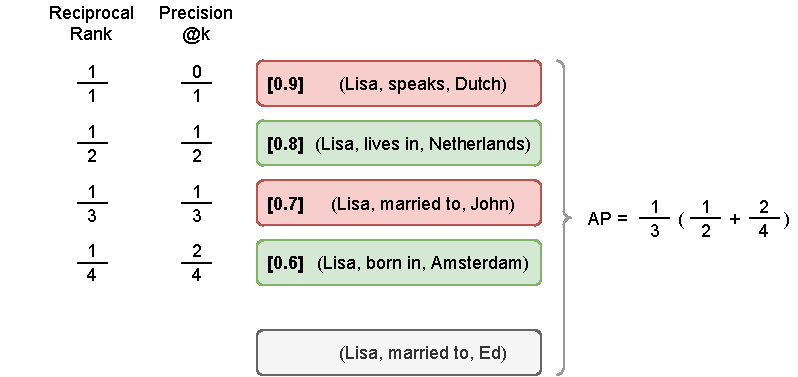
\includegraphics{2_basics/4_metrics/5_map/mrr_map}
    \caption{Calculation of average precision by example of a list of fact predictions, ranked by confidence and containing two of the totally three relevant facts - relevant facts are in green, irrelevant ones in red and the missed out relevant one in grey}
    \label{fig:2_basics/4_metrics/5_map/mrr_map}
\end{figure}

As for the MRR, mAP takes values in $(0, 1]$ and is not defined if there are no relevant items for an object. Again, the latter case might be handled by ignoring such objects. When evaluating $n$ objects, each with $AP_i$ with $1 <= i <= n$, \emph{mean average precision (mAP)} is calculated as the overall average value:

\begin{align}
    mAP = \frac{1}{n} \sum_{i=1}^{n} AP_i
    \label{eq:2_basics/4_metrics/5_map/map}
\end{align}







    \chapter{Related Work}
    \label{ch:3_related_work}
    Not surprisingly, many different approaches to knowledge graph completion have been developed. These can be categorized according to various criteria, such as whether they operate on the pure graph or use auxiliary information, or whether they are primarily aimed at predicting facts or are designed for a downstream task. Furthermore, they can be grouped into symbolic and embedding-based approaches can be distinguished, which also roughly covers their chronological order.

The classical, symbolic approaches consider graphs in their ``natural'' form where entities and relations are distinguishable objects. The standard example of a symbolic approach is a rule miner that finds logical rules that can then be used to predict new facts. The advantages of symbolic approaches are that they require little or no training since they are directly applicable to graphs. Furthermore, they process the symbols in a way that is comprehensible to humans, which also allows manually adding domain-specific knowledge. A limitation of distinct symbols is that similarities between them cannot be leveraged easily. For example, rules for the entity $City$ do not automatically apply to the entity $Town$. Another drawback is poor scalability due to long computation times for large graphs.

In contrast to symbolic approaches are the embedding-based approaches that originate from the field of NLP where the concept is used to embed words in a continuous, low-dimensional vector space. Analogously, KGC models embed the entities and relations of a graph using floating-point vectors, which can be processed very efficiently by modern processors. Moreover, similarities between entities and relations can be covered. For example, the entity $City$ could be assigned a similar embedding as $Town$. Then, when processing $Town$-related knowledge, there is a good chance that patterns related to $City$ can be used. One disadvantage of embedded entities is that they must first be trained extensively until they reach their desired relative position to other embeddings, which requires large amounts of training data. Furthermore, the learned embeddings are not comprehensible to humans, making it harder to understand the model's decision.

Besides the pure facts of a knowledge graph, in practice, there is often additional information about the entities and relations such as textual descriptions that can be used in KGC. In particular, such additional information enables the support of open-world scenarios in which predictions shall be made for entities for which no facts exist are known.

In the following, \autoref{sec:3_related_work/1_symbolic} reviews symbolic approaches -- in particular the rule-based approach relevant to this work. Subsequently, \autoref{sec:3_related_work/2_embedding_based} gives an overview of different approaches of the widespread, state-of-the-art embedding-based models. Finally, \autoref{sec:3_related_work/3_additional_information} shows how embedding-based models incorporate additional information, such as textual entity descriptions, to improve performance before \autoref{ch:4_approach} continues to explain how the model uses additional information in combination with a rule-based model.


\section{Symbolic}
\label{sec:3_related_work/1_symbolic}
The classical, symbolic approach to knowledge graph completion consists of capturing patterns in the graph structure in the form of logical rules. An example of a rule would be $(X, lives~in, Netherlands) <= (X, born~in, Amsterdam)$, which states that a person born in Amsterdam lives in the Netherlands. Rules do not express absolute truths but are associated with confidences that indicate how reliable they are. For reasons of computability and runtime complexity, many rule miners restrict themselves to finding Horn rules. Although Horn rules cannot express any logical pattern, they are sufficient in practice.

The concept of logical rules is not new and has been used in inductive logic programming (ILP)~\cite{Muggleton1994InductiveLP}, such as ALEPH~\cite{ALEPH}, for a long time. However, ILP approaches do not scale very well with the size of modern knowledge graphs and mostly require negative examples, which are not given under the open-world assumption. This is addressed by modern approaches such as the \emph{top-down} rule miner AMIE~\cite{Galrraga2013AMIEAR} and its successor AMIE+~\cite{Galrraga2015FastRM} or the \emph{bottom-up} rule miner AnyBURL~\cite{Meilicke2019AnytimeBR}, which is used in this work. Thereby, top-down algorithms start their search for rules with general rules they try to find evidence for, while bottom-up approaches start with concrete paths in the graph which they try to generalize to rules.

Another way to find rules is \emph{differentiable rule mining}, implemented by neural theorem provers (NTPs)~\cite{Rocktschel2017EndtoendDP}, DRUM~\cite{Sadeghian2019DRUMED} and Neural LP~\cite{Yang2017DifferentiableLO}. These models represent rules numerically and thus enable end-to-end learning of rules. To represent a rule numerically, they encode a rule's facts as $|E| \times |E|$ matrices, that state which head entity $head \in E$ is connected to which tail entity $tail \in E$ by setting a $1$ in the matrix' respective cell. A rule is then represented by the $|E| \times |E|$ matrix calculated as the product of its facts' matrices. A limitation of the listed models is that they can only represent path-like rules.

An alternative symbolic approach to rule mining is the usage of \emph{description logics (DLs)}~\cite{Baader2003TheDL} to form so-called \emph{axioms} that capture patterns in the graph, which also have the advantage of being understandable to humans. An example of an axiom would be $Belgian \sqsubseteq DutchSpeaker \sqcup FrenchSpeaker$. As one can guess from the similarity to set operators, the axiom states that Belgians speak either Dutch, French, or both. Just like rules, those axioms are not inherently true but hold with a certain confidence. The mentioned axiom, for example, does not consider German-speaking Belgians. Two concrete axiom miners are the ones created by Völker et al.~\cite{Vlker2015AutomaticAO} and Töpper et al.~\cite{Tpper2012DBpediaOE}.



\section{Embedding-Based}
\label{sec:3_related_work/2_embedding_based}
Most of the current, state-of-the-art knowledge graph completion models are based on the idea that the objects of interest can be embedded as low-dimensional, numerical vectors that can be computed effectively and efficiently by downstream models as proven in multiple other fields in the recent past, such as NLP and image processing~\cite{Wang2017KnowledgeGE}. Thereby, low-dimensional referrs to vectors limitted to a few hundred dimensions, which is low compared to comparable one-hot encodings. Equivalent to words in NLP and images in image processing, the embedded objects in KGC are a knowledge graph's entities and relations, although in practice many KGC models merely embed a graph's entities directly, while the relations' embeddings are implied, for example by the entities' relative positions to each other.

The overall process by which meaningful embeddings are created often starts with randomly initializing entity embeddings - and relation embeddings if they are represented explicitly. During training, a KGC model then repeatedly calculates the probability of facts using a scoring function that takes a fact's entity and relation embeddings as input. Thereby, the training objective is to rearrange the entity and relation embeddings so that the scoring function produces high probabilites for true facts and low probabilites for wrong facts. That rearrangement is performed by minimizing a loss function, that could be the negative of the scoring function, using backpropagation. Although most approaches see the graph under the open-world assumption, many support training by producing false facts artificially, known as \emph{negative sampling}, by corrupting true facts, i.e. replacing a true facts head or tail entity with another, random entity. Thereby, chances are high to generate a truly false fact that helps with discriminating true and false facts. At the end of training, the knowledge graph is embedded in a way that captures the structure of the original graph and can be used for further reasoning via cheap vector operations.

Various KGC models differ in their choice of a concrete embedding space, whether and how they embed relations as well as the kind of scoring function they use. As for the embedding space, many models embed the graph in a real-valued, euclidean space, whereas other models chose complex or non-euclidean spaces. Concerning relations, some models embed them implicitly as the relative position between entity embeddings, while others assign vectors, matrices or even tensors to each relation. Finally, models differ in whether they use a distance-based or a similarity-based scoring function. Overall, embedding-based KGC models can be roughly grouped into translational, tensor decomposition, neural and language models.

\begin{figure}[t]
    \centering
    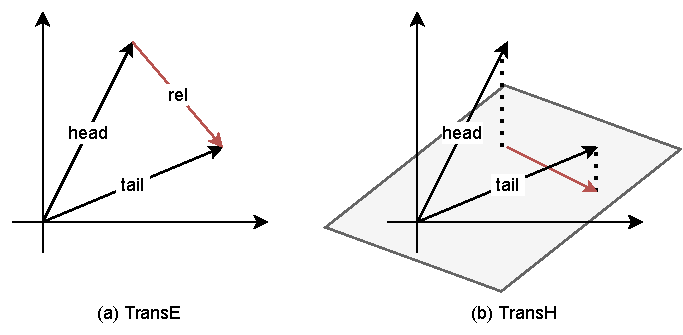
\includegraphics{3_related_work/2_embedding_based/translational}
    \caption{Concept behind translational KGC models: Relations are implicitly represented as vectors between entities - either (a) directly, as for TransE, or (b) indirectly, as for TransH, which projects entity embeddings to relation-specific hyperplanes before performing translation, which supports more complex relations.}
    \label{fig:3_related_work/2_embedding_based/translational}
\end{figure}

From the different kind of models, translational models might be the most intuitive ones. The first and simplest one is TransE~\cite{Bordes2013TranslatingEF} whose basic idea is similar to the concept behind the language model word2vec~\cite{Mikolov2013EfficientEO}: Just like the latter embeds words such that differences between word embeddings reflect semantic relations, TransE embeds entities so that differences between entity embeddings imply relations between them. For example, in word2vec the vector between the word embeddings "king" and "man" is similar to the vector between "queen" and "woman". Analogously, in the embedding space learned by TransE, one might get from the entity embedding of "king" to the entity embedding of "man" by adding the embedding of the relation "is royal" to the entity "king". Figure~\ref{fig:3_related_work/2_embedding_based/translational} illustrates the concept. Formally, given a fact $(\textbf{head}, \textbf{rel}, \textbf{tail})$, TransE learns embeddings such that $\textbf{head} + \textbf{rel} \approx \textbf{tail}$ if the fact is true and $\textbf{head} + \textbf{rel} \neq \textbf{tail}$ if not. It thus minimizes a loss function that aims at maximizing the score function, which is the negative distance between the predicted and the actual tail embedding:

\begin{align}
    score(\textbf{head}, \textbf{rel}, \textbf{tail}) = {- || \textbf{head} + \textbf{rel} - \textbf{tail} ||}_{2}
    \label{eq:3_related_work/2_embedding_based/trans_e}
\end{align}

Problems with TransE's simple approach arise when it comes to 1-n, n-1 and n-m relations. For example, representing the facts $(Ed, speaks, Dutch)$ as well as $(John, speaks, Dutch)$ would require the entities of Ed and John to be roughly at the same spot in embedding space, but other relations between the two might require them to be apart from each other. Also problematic are cyclic relations, such as "married to", because TransE learns that all relations are represented by a vector of zeros. This is where other translational models step in. TransH~\cite{Wang2014KnowledgeGE}, for example, maps the entities onto relation-specific hyperplanes as illustrated in Figure~\ref{fig:3_related_work/2_embedding_based/translationa} before performing the translation. That way multiple entities can be projected onto the same spot on the hyperplane without being at the same location in space. Similarly, TransR~\cite{Lin2015LearningEA} maps entity embeddings into separate, relation-specific embedding spaces, while other models like RotatE~\cite{Sun2019RotatEKG} and MuPR~\cite{Balazevic2019MultirelationalPG} take another approach and work in complex or hyperbolic embedding spaces, which provide "enough room" for the respective relations.

\begin{figure}[t]
    \centering
    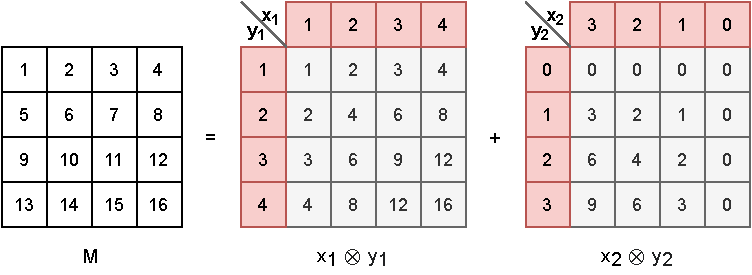
\includegraphics{3_related_work/2_embedding_based/tensor_decomposition}
    \caption{Example for tensor decomposition: A high-dimensional tensor (here, the matrix $M$) can be approximated as the sum of outer products of lower-dimensional tensors (here, the vectors $x_1$, $y_1$, $x_2$ and $y_2$).}
    \label{fig:3_related_work/2_embedding_based/tensor_decomposition}
\end{figure}

Different from translational KGC models, tensor decomposition models are based on the idea that the graph embedding space can be expressed as a composition of many smaller tensors that represent entities and relations. Figure~\ref{fig:3_related_work/2_embedding_based/tensor_decomposition} demonstrates tensor decomposition by an example: A matrix, which is a two-dimensional tensor, can be calculated as the sum of two outer vector products between four vecctors, which are one-dimensional tensors. Likewise, a graph $G$ can be approximated by $3 \times d$ d-dimensional vectors:

\begin{align}
    G \approx \sum_{i=1}^{d} \textbf{x}_i \otimes \textbf{y}_i \otimes \textbf{z}_i
    \label{eq:3_related_work/2_embedding_based/tensor_decomposition}
\end{align}

The mathematics behind tensor decomposition can then be used to optimize the similarity-based scoring function of tensor decomposition models. For example, Equation~\ref{eq:3_related_work/2_embedding_based/distmult} shows the score function of DistMult~\cite{Yang2015EmbeddingEA}, which corresponds to optimizing a tensor decomposition where entities and relations are represented by d-dimensional vectors.

\begin{align}
    score(\textbf{head}, \textbf{rel}, \textbf{tail}) = \sum_{i=1}^{d} \textbf{head}_i \cdot \textbf{rel}_i \cdot \textbf{tail}_i
    \label{eq:3_related_work/2_embedding_based/distmult}
\end{align}

Again, the goal of training is to find embeddings that maximize the scoring function for true facts and minimize it for false facts. Thereby, one limitation of DistMult is that its relation vectors cannot capture asymmetric relations. Other models follow different attempts to solve this problem. For example, RESCAL~\cite{Nickel2013TensorFF} represents relations using matrices instead of vectors, HolE~\cite{Nickel2016HolographicEO} leverages the non-comulativity of the correlation operators, ComplEx~\cite{Trouillon2016ComplexEF} works in complex space, and TuckER~\cite{Balazevic2019TuckERTF} employs Tucker decomposition.

\begin{figure}[t]
    \centering
    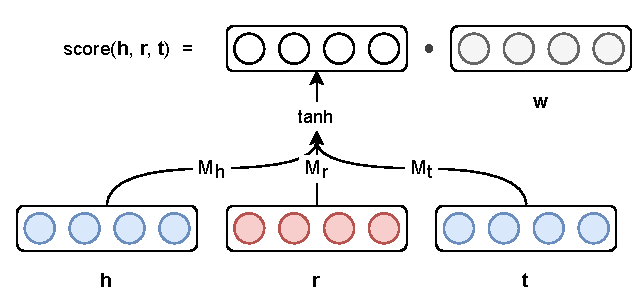
\includegraphics{3_related_work/2_embedding_based/mlp}
    \caption{Architecture of the neural MLP model~\cite{Dong2014KnowledgeVA}. In the first layer, a fact $(\textbf{h}, \textbf{r}, \textbf{t})$ is embedded using three matrices for head, relation and tail embeddings as well as the non-linear $\tanh$ function. In the second layer, the fact's score is calculated as the scalar product of the fact embedding and a weight vector $w$.}
    \label{fig:3_related_work/2_embedding_based/mlp}
\end{figure}

Yet nother approach towards KGC is followed by neural models like MLP~\cite{Dong2014KnowledgeVA} that leverage a non-linear function in a neural net to capture complex relations. Figure~\ref{fig:3_related_work/2_embedding_based/mlp} depicts the two-layer architecture of the MLP model. At the first layer, it multiplies entity and relation vectors with three matrices it keeps for head entities, relations and tail entities before it applies the non-linear $\tanh$ activation function to the sum of resulting vectors. In the second layers follows a simple scalar multiplication with a weight vectors, yielding the final score function:

\begin{align}
    score_{MLP}(\textbf{h}, \textbf{r}, \textbf{t}) = \langle tanh(M_h \cdot \textbf{h} + M_r \cdot \textbf{r} + M_t \cdot \textbf{t}), \textbf{w} \rangle
    \label{eq:3_related_work/2_embedding_based/mlp}
\end{align}

Similar approaches include SME~\cite{Glorot2013ASM}, one of the first models to use a neural network, NTN~\cite{Socher2013ReasoningWN}, which uses relation-wise tensors before applying the non-linear function, and NAM~\cite{LIU2016ProbabilisticRV}, which employs more layers in its deep architecture.

Finally, there are KGC approaches that use the achievements of NLP models even more than tranlsational ones like TransE, in that they directly employ language models. The idea is that the variable-length sentences, consisting of words, that a language model expects as input can be replaced with variable-length paths randomly sampled from the graph, whose path segments correspond to words. Two implementations from this category include RDF2Vec~\cite{Ristoski2016RDF2VecRG}, that builds upon the word2vec~\cite{Mikolov2013EfficientEO} language model, and KGloVE~\cite{Cochez2017GlobalRV}, which is based on GloVE~\cite{Pennington2014GloveGV}.



\section{Using Additional Information}
\label{sec:3_related_work/3_additional_information}
The symbolic and embedding-based approaches discussed so far purely rely on a knowledge graph's fact for prediction. This section presents models that leverage additional information, such as type information, textual entity descriptions or logical rules to improve predictions.

Type information is provided by some knowledge graphs to distinguish between different kinds of entities. A graph representing a social network, for example, might label entities as persons, locations or events. A simple model that leverages such type information is SSE~\cite{Guo2015SemanticallySK}, which keeps entities of the same type closer together during training. One of its drawbacks, however, is that it can only handle non-hierarchical types. In contrast TKRL~\cite{Xie2016RepresentationLO} extends on this and support hierarchical types as well as multiple type labels per entity. Another advantage of typed knowledge graphs is that types can be used to improve negative sampling: By excluding augmented negative samples with correct typings it can be guaranteed that no true facts are generated.

Another kind of additional information, and arguably the most comprehensive one, is textual entity descriptions. Dictionaries and encyclopedias contain concise definitions and descriptions for a wide range of entities and web crawlers can collect texts from vast online sources. The NTN~\cite{Socher2013ReasoningWN} model mentioned before was one of the first KGC models to leverage that information to initialize its entity embeddings by averaging the word embeddings of the entities' names. Similarly Long et al. used longer text descriptions to initialize entity embeddings~\cite{Long2016LeveragingLR}. However, both approaches have in common that the texts are not used to improve fact embeddings during training.

One of the earliest approaches to use texts beyond entity initialization was proposed by Wang et al~\cite{Wang2014KnowledgeGE}. who implemented joint embedding of facts and texts. Later, DKRL~\cite{Xie2016RepresentationLO}, an extension to TransE, and OWE~\cite{Shah2019AnOE}, an extension to embedding-based KGC models in genearl, have been developed. Both have the advantage that they can also be applied to open-world entities that are not seen during training. Figure~\ref{fig:3_related_work/3_additional_information/owe} illustrates the working of OWE: First, word embedding and graph embedding models are trained individually on the text and graph data. Then, an alignment function is learned that maps word embeddings to their respective entity embeddings. This allows texts of open-world entities to be mapped to the right position in the graph embedding space. In the example in Figure~\ref{fig:3_related_work/3_additional_information/owe} it would thus be possible to predict similar facts for the open-world entity John as for the known entity Ed it is close to.

\begin{figure}[t]
    \centering
    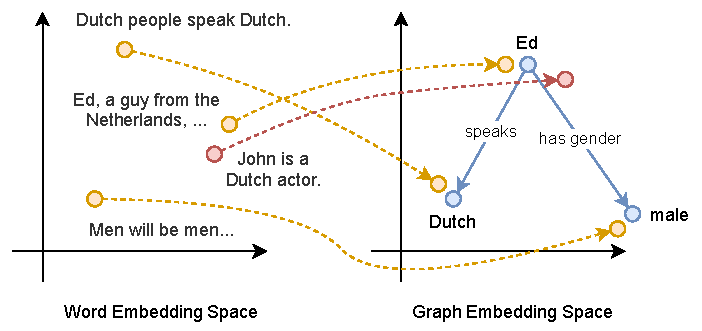
\includegraphics{3_related_work/3_additional_information/owe}
    \caption{The OWE model~\cite{Shah2019AnOE} learns a mapping function to align its separately learned word and graph embedding spaces, which allows predictions for open-world entities. Here, the text of the open-world entity John (red) is embedded close to the text of the known entity Ed, leading to similar embeddings in the graph embedding space, allowing OWE to predict similar facts for John.}
    \label{fig:3_related_work/3_additional_information/owe}
\end{figure}

Finally, beyond type and text information, some models also attempted to incorporate rules into training of embedding-based models. Some early approaches~\cite{Wang2015KnowledgeBC, Wei2015LargescaleKB} used them to put constraint on their predicted facts, but such a post-processing step does not help with training the actual graph embedding. The KALE model~\cite{Guo2016JointlyEK} on the other hand represents facts and rules in a common vector space. The basic idea is to ground the rules and calculate the rule groundings' embeddings from the facts they consist of using fuzzy logics. The probability of a fact $(h, r, t)$ is thereby based on the Manhatten distance between the $d$-dimensional vectors $h + r$ and $t$ as per Equation~\cite{eq:3_related_work/3_additional_information/kale_fac}, while Equation~\ref{eq:3_related_work/3_additional_information/kale_rule} gives an example of how the probability of a rule grounding with two body facts $f_1$ and $f_2$ and a head fact $f_3$ is calculated.

\begin{align}
    I(\textbf{h}, \textbf{r}, \textbf{t}) &= 1 - \frac{1}{3 \sqrt {d}} {|| \textbf{h} + \textbf{r} - \textbf{t} ||}_1
    \label{eq:3_related_work/3_additional_information/kale_fact} \\
    I(f_1 \land f_2 \Rightarrow f_3) &= I(f_1) \cdot I(f_2) \cdot I(f_3) - I(f_1) \cdot I(f_2) + 1
    \label{eq:3_related_work/3_additional_information/kale_rule}
\end{align}

Beyond Horn rules, KALE can handle any propositional logic rules. Given the formula for calculating an arbitrary rule's probability, which includes single facts, KALE then employs a margin-based ranking loss to learn the common embedding space that allows looking up ground path rules that are similar to facts and vice versa. The only drawback is that KALE cannot handle quantifiers from first order logic, which is why it uses rule groundings.




    \chapter{Approach}
    \label{ch:4_approach}
    As described in the introduction in \autoref{ch:1_introduction}, the Power model is an ensemble model, consisting of a rule-based and a text-based component, whose goal is the comprehensible prediction of new facts. Given a query entity with a few known facts and descriptive texts, Power implements this requirement by providing prioritized lists of rules and sentences that were crucial for the predicted facts. Considering the application scenario in which a user uses the model for support of manual knowledge graph completion, it is also important that correct predictions are ranked as high as possible among an entity's predicted facts.

Technically, the Power ensemble consists of three components as shown in \autoref{fig:4_approach/power_architecture}. Besides the rule-based component, named \emph{Ruler}, and the text-based component, named \emph{Texter}, it also contains the so-called \emph{Aggregator} that combines the Ruler's and Texter's predictions. If both Ruler and Texter predict a fact, the final prediction yielded by the Aggregator comes with both, the Ruler's prioritized list of decisive rules and the Texter's ranked list of sentences, and is considered more reliable than a fact predicted by only one of the components.

\begin{figure}[t]
    \centering
    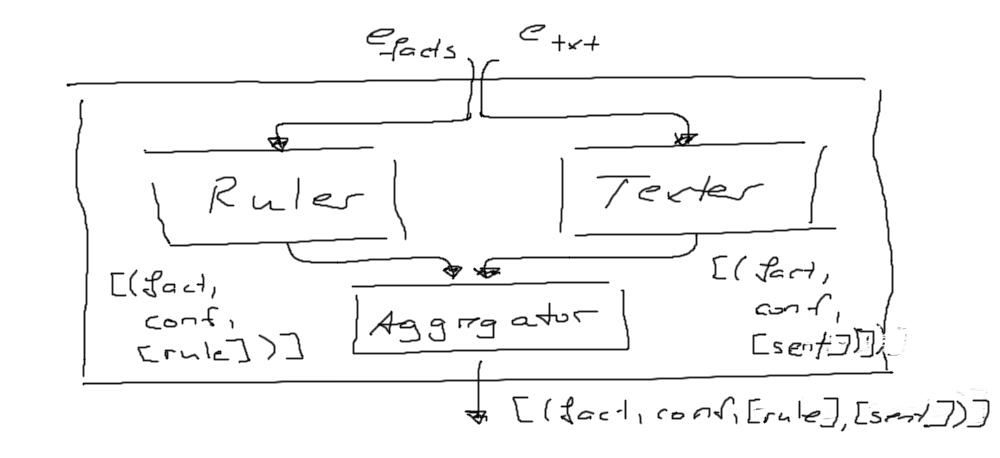
\includegraphics[width=\textwidth]{4_approach/power_architecture}
    \caption{Power model consisting of the Ruler, which processes a query entity's known facts, the Texter, which processes the entity's texts, and the Aggregator, which combines all predictions. All prediction lists are sorted by confidence and come with sorted lists of explaining rules and texts.}
    \label{fig:4_approach/power_architecture}
\end{figure}

Depending on the dataset at hand, either the Ruler or Texter might perform better. In general, the Texter should perform better for graphs that contain many similar facts, such as $(x, part~of, Asia)$ with $x \in \{China, India, Japan, \dots\}$, while the Ruler also works well on diverse datasets but cannot handle open-world entities. Together, they complement each other: The Ruler handles very rare facts while the Texter can bootstrap the prediction process on open-world entities until the Ruler can join when some facts are available for rule application. In \autoref{sec:5_experiments/5_aggregator}, the Ruler's and Texter's evaluation results are compared to each other as well as to the results achieved by the Aggregator.

\section{Texter}
\label{sec:4_approach/1_texter}
While the Ruler processes the query entity's known facts, the Texter takes the entity's sentences to predict facts. Although it can only predict the most common facts from the training set, its main advantage is its applicability to open-world entities that come without any known facts about them.

\subsection{Simple Model}
\label{subsec:4_approach/1_texter/1_simple_model}
During inference, the first step of processing a query entity, which is the same for both the simple and the attentive Texter, is embedding the entity's sentences in the embedding block. Thereby, each sentence is processed individually as illustrated in Figure~\ref{fig:4_approach/1_texter/1_simple_model/simple_architecture}: First, the sentence is split into words by the tokenizer, which are handled as integer IDs in further processing. Next, the words are embedded using some NLP approach, which could be a simple lookup table in the simplest case. As the last step in the embedding block, the word embeddings are combined to sentence embeddings in the pooling layer. The resulting sentence embeddings, that capture the sentences' overall meanings, are then passed on to the classification block where each of them is pushed through the neural multi-label classifier which consists of a single linear layer. Another pooling layer then combines the sentence-wise classification logits to the entity's logits. Finally, applying the sigmoid function to the entity's logits yields the class probabilites that state the probabilities of the associated facts about the query entity.

\begin{figure}[t]
    \centering
    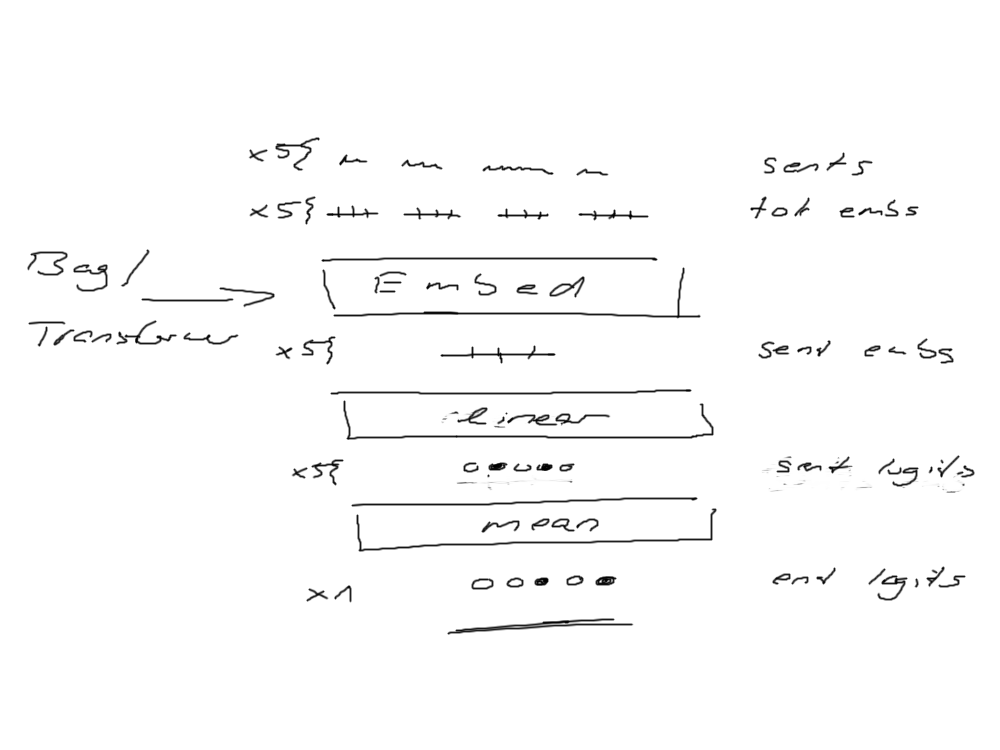
\includegraphics{4_approach/1_texter/1_simple_model/simple_architecture}
    \caption{Simple Texter Architecture; Each sentence is embedded and classified individually before the final pooling layer combines the results; "++++----" represents an embedding with positive and negative elements}
    \label{fig:4_approach/1_texter/1_simple_model/simple_architecture}
\end{figure}

Especially in the embedding block there are different possibilities for the concrete implementation of the individual parts to choose from, some of which will be examined in Chapter~\ref{ch:5_experiments}. In the final version of the power model, a transformer model is used for embedding the sentences' words, more precisely DistilBERT, a "distilled" variant of the transformer encoder BERT reduced to the essentials~\cite{Sanh2019DistilBERTAD}. In contrast to a simple lookup table, DistilBERT is able to incorporate the context of a word into its embedding, which leads to more meaningful sentence embeddings. This choice of embedding approach also affects the tokenizer, the pooling layer, and even the input sentences: Thanks to context embedding, transformers can use special tokens that add additional information to the text. While a classical model cannot decide on the basis of the sentence "Lisa likes John." whether this sentence speaks for the class $(x, has~gender, male)$, a transformer is able to do so given the appropriately marked sentence "Lisa likes [START]John[END].". Especially for long, ambigious sentences performance can be increased significantly.

Beyond the input data, the use of a transformer also affects the tokenizer and the pooling layer. The tokenizer has to apply byte pair encoding (BPE) that is commonly used by pre-trained transformers, where sentences are not only divided into words, but words are further divided into subwords, thus keeping the vocabulary of the tokenizer small and allowing to exploit homorphisms between similar words. In addition, the tokenizer inserts the [CLS] and [SEP] introduced by BERT at the beginning and end of the sentence. That way, "Lisa likes [START]John[END]." becomes "[CLS]Lisa likes [START]John[END].[SEP]". While the [SEP] token is used to separate sentences and has no further meaning here, the embedding of the [CLS] token captures the meaning of the whole sentence and is therefore  used as a sentence representation in the BERT paper~\cite{Devlin2019BERTPO}. However, the power experiments showed that performance can be increased if the word embeddings are also included, which is why the pooling layer of the embedding block averages all of a sentence's token embeddings, including the [CLS] embedding.

Less comprehensive processing steps happen in the classification block of the simple Texter: The sentence embeddings produced by the embedding block are pushed through the single linear classification layer whose multi-label output logits are averaged in the final pooling layer. The class probabilities calculated by applying the sigmoid function to the resulting entity logits are then used to sort the facts that have a probability greater than 50\%. Thus, the user of the model first receives the facts that are most likely to apply.


\subsection{Attention Model}
\label{subsec:4_approach/1_texter/2_attention_model}
While the simple Texter produces good evaluation results and does return a prioritized list of predicted facts, its prediction miss the desired explanation of why a fact is suggested. At this point, the attentive Texter extends the simple model by an attention mechanism that compares an entitiy's sentences to each other, forcing the model to favor sentences that are most relevant to the prediction of a certain fact. Besides the ability to provide an explanations for its predictions, the added attention mechanism should also increase the Texter's performance on datasets with multiple sentences per entity.

Technically, the attention mechanism is implemented as an attention block between the embedding and the classification blocks as shown in Figure~\ref{fig:4_approach/1_texter/2_attention_model/attention_architecture}. The embedding block is the same one used in the simple model, leveraging the DistilBERT encoder's contextual word embeddings to support marked input sentences and produce meaningful sentence embeddings. The classification block still produces the entity's multi-label output logits, but now uses multiple smaller linear layers to do so, due to the different outputs passed in from the attention block.

\begin{figure}[t]
    \centering
    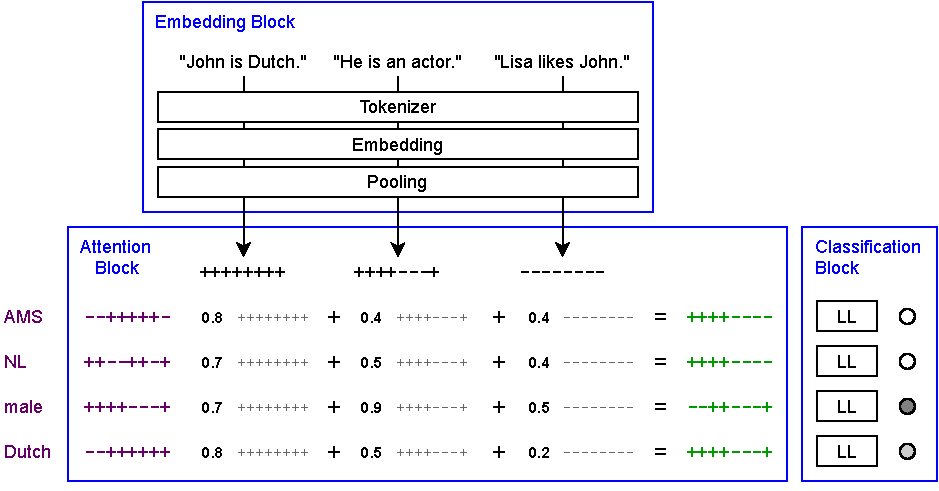
\includegraphics{4_approach/1_texter/2_attention_model/attention_architecture}
    \caption{Texter Architecture}
    \label{fig:4_approach/1_texter/2_attention_model/attention_architecture}
\end{figure}

The attention block now takes the sentence embeddings from the embedding block and compares them to so-called \emph{class embeddings} that represent each of the models output classes as a vector of the same dimension as the sentence embeddings. Given the set of input sentences $S$ and the set of classes $C$, the similarity between a class embedding $class_c$ and a sentence embedding $sent_s$ with $1 <= c <= |C|$ and $1 <= s <= |S|$ is calculated as the scalar product $\langle class_c, sent_s \rangle$ between the class and the sentece embedding. Given all class-sentence similarities for a certain class, the model can decide which sentence is matches the best for that class and deserves most attention when it comes to the decision whether the class holds true. Therefore, those similarity values are also referred to as attention values. To minimize the effect of sentences whose embeddings are very similar to a class embedding by pure chance, the attention values are furthermore normalized using the sigmoid function. Thus, the total attention matrix containing the attention values for all combinations of classes from $C$ and sentences from $S$ is calculated as shown in Equation~\ref{eq:4_approach/1_texter/2_attention_model/attention_matrix}.

\begin{align}
    A_{cs} = \sigma(\langle class_c , sent_s \rangle) && 1 <= c <= |C|, 1 <= s <= |S|
    \label{eq:4_approach/1_texter/2_attention_model/attention_matrix}
\end{align}

In the next step, the calculated attention values are used to combine the sentence embeddings to class-wise entity embeddings $ent_c$. As illstrated in Figure~\ref{fig:4_approach/1_texter/2_attention_model/attention_architecture} and formalized in Equation~\ref{eq:4_approach/1_texter/2_attention_model/ent_emb}, each sentence is thereby weighted by its class-wise attention value. The weighted sentences are then summed up to form class-wise entity embeddings whose purpose is to capture primarily those texts most relevant to the prediction of the respective class. Different from the simple Texter, the entity embeddings are then passed to the subsequent classification block instead of the original sentence embeddings.

\begin{align}
    ent_c = \sum_{s = 1}^{|S|} A_{cs} \cdot sent_s && 1 <= c <= |C|, 1 <= s <= |S|
    \label{eq:4_approach/1_texter/2_attention_model/ent_emb}
\end{align}

Similar to the simple Texter, the attentive Texter's classification consists of a $|C| \times d$ weight matrix and a bias vector of length $d$ where $d$ is the chosen embedding dimensionality for word, sentence, class and entity embeddings. In contrast to the simple model, however, given an entity embedding for a certain class, the weight matrix is not trained with respect to all output classes at once, but only with respect to the regarded class' ground truth output as illustrated in Figure~\ref{fig:4_approach/1_texter/2_attention_model/multi_linear}, which conceptually can be seen as training a separate single-output linear layer for each class and combining the outputs to the multi-label output thereafter. Formally, the models output classification outputs can be calculated as $out_c = \langle ent_c, W_c \rangle + b_c$ where $W_c$ and $b_c$ are the class' row in the weight matrix and its bias, respectively. The described approach to training the weight matrix was chosen, because a certain class' entity embedding focuses on the prediction of a single output class and would only hinder the learning process for other output classes it cannot make a qualified statement about.

\begin{figure}[t]
    \centering
    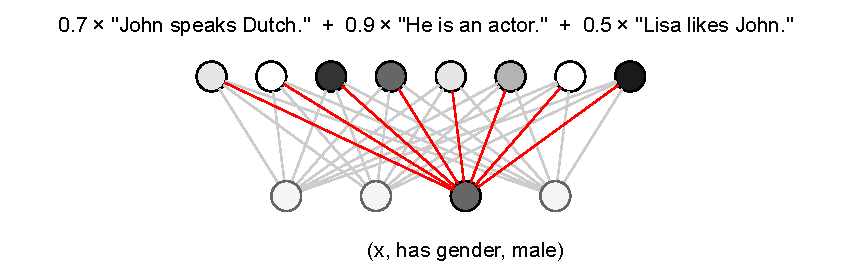
\includegraphics{4_approach/1_texter/2_attention_model/multi_linear}
    \caption{Multi-linear}
    \label{fig:4_approach/1_texter/2_attention_model/multi_linear}
\end{figure}

Similar to the simple Texter, following the core steps, the attentive Texter takes all classes whose confidences, that result from applying the sigmoid function to the output logits, is greater than 50\% to form their corresponding facts and sort them by confidence. In addition to the simple Texter, however, the attentive model provides the facts with the sentence weights as they result from the attention matrix in order to provide the user with an explanation for each fact's prediction. So, in the example, the fact $(John, has~gender, male)$, with a probability around 70\%, would be accompanied by the information that it was primarily suggested due to the sentence "He is an actor.", followed by "John speaks Dutch." and lastly "Lisa likes John.".

learnable class embs
sigmoid maps to (0, 1)
attention matrix A
total number of learnable params
in experiments: applied by an AdamW optimizer, a variant of the Adam optimizer that overcomes Adam's that keeps the training speed of Adam while keeping SGD's superior ability to generalize~, \cite{Loshchilov2019DecoupledWD}




\section{Ruler}
\label{sec:4_approach/2_ruler}
While the Texter processes the text information attached to the knowledge graph's entities, the Ruler exploits patterns in the graph structure to predict missing facts. Given an entity $x$ with a set of known facts $K$ containing facts of the form $(x, rel_k, tail_k)$ with $1 <= k <= |K|$ and $rel_k \in R$ and $tail_k \in E$ being any relation or entity, respectively, the Ruler leverages entity-related rules of the form $(x, rel_m, tail_m) <= (x, rel_k, tail_k)$ with $1 <= m <= |M|$ to predict a set of missing facts $M$. Therefore, the rules required for the inference process have to be mined from the knowledge graph, beforehand. That rule mining process can be viewed as the equivalent to the Texter's training process and some paragraphs in this thesis will refer to combined rule mining and creation of a Ruler as "training" a Ruler. Compatibel to the Texter, the Ruler is limited to the prediction of facts $(x, rel, tail)$ that contain the query entity as their head, as well. However, when the Ruler is applied to all entities $e \in E$, all facts of the form $(e, rel, x)$ are predicted at some point as far as the mined rules support it.

For rule mining, AnyBURL, the bottom-up rule mining algorithm, by Christian Meilicke et al.~\cite{Meilicke2019AnytimeBR} is used. It is an anytime algorithm, meaning that it can be interrupted anytime and still yield valid results. Bottom-up rule mining refers to the fact that the algorithm starts with concrete paths in the graph and tries to generalize those paths to rules instead of coming up with rules initially and searching for evidence later, which would be a top-down approach. Out of all possible Horn rules that might describe patterns in the graph, AnyBURL is restricted to rules that can be generalized from so-called \emph{ground path rules}. A ground path rule does not contain variables, but only constants, and must not contain any cycles in its body. Equation~\ref{eq:4_approach/2_ruler/ground_path_rule} describes the general form of a ground path rule of length $n$, meaning that it consists out of the head fact and $n$ body facts.

\begin{align}
(c_0, h, c_1)
    \Leftarrow (c_1, b_1, c_2), \dots, (c_n, b_n, c_{n+1}) &&
    c_k \neq c_l \forall k, l \in \{1, \dots, n+1\}, k \ne l
    \label{eq:4_approach/2_ruler/ground_path_rule}
\end{align}

Notably, despite the rule body being free of cycles, the ground path rule as a whole can still be cyclic if $c_0 = c_{n+1}$. Ground path rules are derived directly from randomly sampled paths in the graph and are subsequently generalized to rules that replace some of the constants with variables. If further supporting paths can be found for a general rule, it is kept. In their paper on AnyBURL, Meilicke et al. show that any rule that can be generalized from a ground path rules can be generalized to one of the three rule types formulated in Equations~\ref{eq:4_approach/2_ruler/c}~--~\ref{eq:4_approach/2_ruler/ac2}. Thereby, $C$-type rules can only be generalized from cyclic ground path rules, $AC2$ rules can only be generalized from acyclic ground path rules and $AC1$ can be generalized from both, cyclic and acyclic ground path rules. The following paragraphs outline the core algorihm used to mine such rules and derive some example rules from the small graph introduced in Chapter~\ref{ch:1_introduction}. Figure~\ref{fig:4_approach/2_ruler/rule_graph} shows an annotated subset of the graph that illustrates the rules. "Amsterdam" and "Netherlands" have been abbreviated to "AMS" and "NL" to keep the examples short.

\begin{align}
    C   && (Y, h, X)   &\Leftarrow (X, b_1, A_2), \dots, (A_n, b_n, Y)
    \label{eq:4_approach/2_ruler/c} \\
    AC1 && (c_0, h, X) &\Leftarrow (X, b_1, A_2), \dots, (A_n, b_n, c_{n+1})
    \label{eq:4_approach/2_ruler/ac1} \\
    AC2 && (c_0, h, X) &\Leftarrow (X, b_1, A_2), \dots, (A_n, b_n, A_{n+1})
    \label{eq:4_approach/2_ruler/ac2}
\end{align}

\begin{figure}[t]
    \centering
    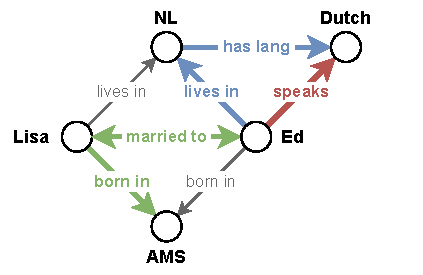
\includegraphics{4_approach/2_ruler/rule_graph}
    \caption{Subset of the previously introduced example graph with highlighted facts that form an acyclic (red + green) and a cyclic (red + blue) path.}
    \label{fig:4_approach/2_ruler/rule_graph}
\end{figure}

Essentially, AnyBURL repeatedly samples random paths from the graphs, generalizes them to all possible rule types, looks for further paths that match the gained rules, and keeps those rules it finds further evidence for. For example, in search of rules of length 2, i.e. rules that have a body consisting of 2 facts, AnyBURL might randomly sample the two paths in~\ref{eq:4_approach/2_ruler/path_1} and~\ref{eq:4_approach/2_ruler/path_2} from the graph. Note, that parentheses denote entities, brackets denote relations and that the path does not need to follow directed edges in the graph. Furthermore, a close look at the paths reveals that the second path is cyclic as it starts and ends at the entity "Dutch".

\begin{align}
(Dutch)
    \leftarrow [speaks] - (Ed) - [married~to] \rightarrow (Lisa) - [born~in] \rightarrow (AMS)
    \label{eq:4_approach/2_ruler/path_1} \\
    (Dutch) \leftarrow [speaks] - (Ed) - [lives~in] \rightarrow (NL) - [has~lang] \rightarrow (Dutch)
    \label{eq:4_approach/2_ruler/path_2}
\end{align}

From those paths, AnyBURL would then derive the constant-only
ground path rules~\ref{eq:4_approach/2_ruler/acyclic_ground_path} and~\ref{eq:4_approach/2_ruler/cyclic_ground_path} by taking the path's first part as the rule's head and the remaining parts to form the rule's body.

\begin{align}
(Ed, speaks, Dutch)
    &\Leftarrow (Ed, married~to, Lisa), (Lisa, born~in, AMS)
    \label{eq:4_approach/2_ruler/acyclic_ground_path} \\
    (Ed, speaks, Dutch) &\Leftarrow (Ed, lives~in, NL), (NL, has~lang, Dutch)
    \label{eq:4_approach/2_ruler/cyclic_ground_path}
\end{align}

The acyclic ground path rule in~\ref{eq:4_approach/2_ruler/acyclic_ground_path} can be generalized to the $AC1$ rule~\ref{eq:4_approach/2_ruler/acyclic_ac1} and the $AC2$ rule~\ref{eq:4_approach/2_ruler/acyclic_ac2} while the cyclic ground path rule~\ref{eq:4_approach/2_ruler/cyclic_ground_path} can be generalized to the $C$ rule~\ref{eq:4_approach/2_ruler/cyclic_c} and the $AC1$ rule~\ref{eq:4_approach/2_ruler/cyclic_ac1}.

\begin{align}
    AC1 && (X, speaks, Dutch) &\Leftarrow (X, married~to, A_2), (A_2, born~in, AMS)
    \label{eq:4_approach/2_ruler/acyclic_ac1} \\
    AC2 && (X, speaks, Dutch) &\Leftarrow (X, married~to, A_2), (A_2, born~in, A_3)
    \label{eq:4_approach/2_ruler/acyclic_ac2} \\
        C   && (X, speaks, Y) &\Leftarrow (X, lives~in, A_2), (A_2, has~lang, Y)
    \label{eq:4_approach/2_ruler/cyclic_c} \\
    AC1 && (X, speaks, Dutch) &\Leftarrow (X, lives~in, A_2), (A_2, has~lang, Dutch)
    \label{eq:4_approach/2_ruler/cyclic_ac1}
\end{align}

Next, every rule candidate is scored by looking for further paths that match the rule's body and checking whether the graph also contains the fact predicted by the rule, i.e. whether the rule is correct in that case. Thereby, the number of paths that match the rule body is called the rule's \emph{support} while the ratio of times the rule is correct over its total support is called \emph{confidence}. Taking the cyclic rule~\ref{eq:4_approach/2_ruler/cyclic_c} as an example, AnyBURL would search for further evidence and find the path $(Lisa) - [lives~in] -> (NL) - [has~lang] -> (Dutch)$ that matches the rule body, increasing the rule's support to two, so far. However, the example graph does not contain the rule's predicted fact $(Lisa, speaks, Dutch)$, so the rule's support drops from 1 to $\frac{1}{2}$. Since rules that only apply to a single case or only once in every thousands case are not very useful, AnyBURL drops rules with a support of 1 or confidence below 0.0001 by default~\cite{AnyBURL}. It is noteworthy that, although some rules are more general than others, such as~\ref{eq:4_approach/2_ruler/acyclic_ac2} compared to~\ref{eq:4_approach/2_ruler/acyclic_ac1}, the more specific ones are still kept as they might end up with higher confidence for their special case during the ongoing mining process.

The process described by the above example is repeated until only few new rules of the same length $n$ can be found. AnyBURL then continues its search for rules of length $n + 1$ until it terminates after a fixed number of time steps. Listing~\ref{code:anyburl} shows the slightly adjusted pseudocode from the AnyBURL paper. The sampling and scoring process discussed above is implemented as the body of the inner while loop. The outer for loop implements the repeated check for the saturation of rules of the current length and the eventual proceeding to rules of increased length.

% TODO param s

\begin{listing}[t]
    \begin{lstlisting}
        AnyBURL(G, sat, Q, i, ts):
            n = 2
            R = $\emptyset$
            for i times:
                $R_s = \emptyset$
                start = current_time()
                while current_time() < start + ts:
                    p = sample_path(G, n)
                    $R_p$ = generate_rules(p)
                    for $r$ in $R_p$:
                        score($r$)
                        if $Q$($r)$:
                            $R_s$ = $R_s \cup {r}$

                $R_s^{'}$ = $R_s \cap R$
                if $|R_s^{'}| / |R_s| > sat$:
                    n = n + 1
                $R$ = $R \cup R_s$

            return $R$
    \end{lstlisting}
    \caption{The AnyBURL rule mining algorithm takes a graph $G$, a saturation level $sat$, a quality criterion $Q$, and a number of iterations $i$, each of a timespan $ts$, as input and produces a ruleset $R$.}
    \label{code:anyburl}
\end{listing}

A walk through the pseudocode reads as follows: Given the Graph $G$, the saturation threshold $s$, the quality criterion $Q$, a number of iterations $i$ and the timespan $ts$ each iteration endures, AnyBURL starts with an empty ruleset $R$, that will be extended after each iteration and returned in the end. The initial length of the randomly sampled paths is $n=2$, allowing to find the shortest possible rules of length 1. During the first iteration of duration $ts$, AnyBURL fills the rule set $R_s$, that keeps the rules found in the current iteration, by repeatedly sampling paths, generating rules from the paths, scoring the resulting rules, and keeping those with sufficient support and confidence. At the end of the iteration, when the timespan $ts$ has passed, $R_s^{'}$ is calculated as the set of rules mined during the iteration that were already known. If the share of already known rules mined during the current iteration exceeds the saturation threshold, the algorithm starts searching for rules of increased length. Otherwise, it continues with the current length. In both cases, the iteration's rules are added to the overall ruleset $R$. If the specified number of total iterations is reached, AnyBURL terminates and returns the mined rules $R$. In practice, AnyBURL saves the mined rules in a text file at the end and at configurable points during mining.

With the stored rules from AnyBURL in place, the Ruler is prepared for inference. Conceptually, given an entity and its known facts, the Ruler loads the rules, filters out further rules that do not meet the Ruler's quality demands and applies the remaining, useful rules to all known facts. All rules that can be applied successfully are kept together with their confidence. From all the facts predicted by the applied rules, already known facts from the existing graph are filtered out. The remaining facts are sorted by confidence and returned to the user - together with the rules that predicted them as an explanation for the user. If multiple rules predict the same fact, the fact is assigned the highest confidence of those rules and is returned together with all of them. The Ruler's extra quality criterion mentioned above further restricts the considered rules to those with confidence greater 50\%, because AnyBURL's minimum confidence threshold of 0.01\% allows many rules that predict false positives. For open-world entities, this algorithm implies an empty result set as no rule can cover an entity that is not connected to any other entity and all the facts predicted for the train entities will be filtered out. In those cases, the Power model has to rely solely on the Texter.



\section{Aggregator}
\label{sec:4_approach/3_aggregator}
The aggregator has the task of merging the predicted facts from Ruler and Texter. As envisioned in \autoref{sec:4_approach/3_aggregator} and illustrated in \autoref{fig:4_approach/3_aggregator/lucy}, it was hoped that merging the facts leads to higher average precision because facts predicted by both components are likely to be correct and should be ranked higher. In addition, the Aggregator should be able to estimate how reliable the predictions of Ruler and Texter are in relation to each other, which is implemented in the form of the weight parameter $\alpha$ as described in \autoref{eq:4_approach/3_aggregator/conf_aggregator}.

\autoref{tab:5_experiments/5_aggregator/results} shows the final evaluation results for the Aggregator, and thus the final evaluation results for the Power model, for a number of graph-text combinations. As fact splits, the splits with 50\% known test facts were chosen, as for the final Ruler evaluation in \autoref{sec:5_experiments/4_ruler}. The respective results for the CDE-50 and FB-50 splits from \autoref{tab:5_experiments/4_ruler/results} were taken over into \autoref{tab:5_experiments/5_aggregator/results} for easier comparability. Similarly, the chosen text sets are the ones from the final Texter evaluation in \autoref{subsec:5_experiments/3_texter/3_context}. Again, \autoref{tab:5_experiments/5_aggregator/results} duplicates the respective results from \autoref{tab:5_experiments/3_texter/3_context/results} for ease of comparison. The last two columns then contain the new Aggregator measurements for the combination of the corresponding Ruler and Texter.

\begin{table}[t]
    \makebox[\textwidth][c]{
        \begin{tabular}{ l l c r r r }
    \toprule

    \multicolumn{1}{l}{\textbf{Text Set}} &
    \multicolumn{1}{l}{\textbf{Texter}} & \phantom &
    \multicolumn{3}{c}{\textbf{Macro over Classes}} \\

    \cmidrule{4-6}

    & 
    &&
    \multicolumn{1}{c}{\textbf{Prec}} &
    \multicolumn{1}{c}{\textbf{Rec}} &
    \multicolumn{1}{c}{\textbf{F1}} \\
    
    \midrule

    \multirow{2}{*}{cde-cde-1-clean}
    & Simple    && \textbf{49.02} & 47.57 & 47.67 \\
    & Attentive && 46.86 & \textbf{51.09} & \textbf{47.98} \\

    \addlinespace

    \multirow{2}{*}{cde-irt-1-clean}
    & Simple    && 25.20 & \textbf{34.18} & \textbf{28.13} \\
    & Attentive && \textbf{26.70} & 31.41 & 27.43 \\

    \addlinespace

    \multirow{2}{*}{cde-irt-5-clean}
    & Simple    && 36.49 & \textbf{44.38} & \textbf{38.98} \\
    & Attentive && \textbf{39.20} & 37.11 & 36.98 \\

    \addlinespace

    \multirow{2}{*}{cde-irt-15-clean}
    & Simple    && 41.83 & \textbf{48.69} & \textbf{44.07} \\
    & Attentive && \textbf{44.63} & 37.39 & 39.78 \\

    \addlinespace

    \multirow{2}{*}{cde-irt-30-clean}
    & Simple    && 40.73 & \textbf{50.09} & \textbf{44.11} \\
    & Attentive && \textbf{43.60} & 36.10 & 38.78 \\
    
    \midrule

    \multirow{2}{*}{fb-owe-1-clean}
    & Simple    && 42.36 & \textbf{86.72} & 54.03 \\
    & Attentive && \textbf{45.21} & 84.03 & \textbf{56.16} \\

    \addlinespace

    \multirow{2}{*}{fb-irt-1-clean}
    & Simple    && 26.40 & 46.68 & 32.51 \\
    & Attentive && \textbf{27.01} & \textbf{49.90} & \textbf{34.26} \\

    \addlinespace

    \multirow{2}{*}{fb-irt-5-clean}
    & Simple    && 34.37 & \textbf{55.95} & 40.88 \\
    & Attentive && \textbf{39.21} & 50.63 & \textbf{43.50} \\

    \addlinespace

    \multirow{2}{*}{fb-irt-15-clean}
    & Simple    && \textbf{48.95} & \textbf{54.85} & \textbf{50.06} \\
    & Attentive && 48.89 & 52.75 & 49.92 \\

    \addlinespace

    \multirow{2}{*}{fb-irt-30-clean}
    & Simple    && 43.90 & \textbf{63.31} & \textbf{50.55} \\
    & Attentive && \textbf{50.57} & 48.47 & 48.79 \\
    
    \bottomrule
\end{tabular}

    }
    \caption{Final Aggregator results, i.e. final results for the Power model. The results of the Ruler and Texter, whose predictions the Aggregator combines, are also shown for comparison. Although the Aggregator does not outperform its respective Ruler and Texter in terms of F1 score, it does for mAP.}
    \label{tab:5_experiments/5_aggregator/results}
\end{table}

As the mAP values show, the Aggregator performs several percentage points better than the Ruler and Texter on their own, with the improvement on the CDE split being more obvious. However, the relatively small increase on the FB split suggests that the true positives of Ruler and Texter almost coincide there. For the CDE split, on the other hand, manually peeking into the predictions reveals that the improved mAP mainly results from complementary true positives -- and not so much from improved ranks of joint predictions. Looking at the values of simple and attentive Texter, it is also noticeable that the lead of the simple Texter over the attentive Texter shrinks when adding the Ruler. Likewise, the lead of the text sets with many sentences and with high-quality sentences shrinks. Finally, the different aptitudes for Ruler and Overall, the Aggregator results are even similar between the two splits, while previously, models performed significantly better on the FB split.

Two experiments that will be mentioned only briefly here, because of their unspectacular results, concerning the calculation of the Aggregator's confidence as per \autoref{eq:4_approach/3_aggregator/conf_aggregator}: First, in the beginning, experiments were conducted on the computation of the combined confidence $conf_{Aggregator}$ in cases where facts are predicted by Ruler and Texter. As combining methods, calculating the maximum and the mean of $conf_{Ruler}$ and $conf_{Texter}$ were evaluated, but it soon became apparent that summing them up much better accommodates the fact that a fact predicted by Ruler and Texter deserves very high confidence. Second, experiments showed that taking into account the weight parameter $\alpha$ between Ruler and Texter yields only marginal performance improvements in the tenths of a percent range because the confidence values of Ruler and Texter seem to be very comparable after all and thus always yield $\alpha$ values close to 0.5. In detail, Ruler and Texer were both a bit too optimistic about their predictions in the experiments -- but they were equally overconfident.




    \chapter{Experiments}
    \label{ch:5_experiments}
    \autoref{ch:4_approach} has presented the Power model consisting of the Texter, Ruler and Aggregator components. This chapter presents the evaluation results and experiments performed on data originating from two knowledge graphs and various text sources. \autoref{sec:5_experiments/1_data_sources} introduces the considered knowledge graphs and text sources, followed by \autoref{sec:5_experiments/2_power_splits} that presents the \emph{Power datasets} created from those, which in turn were used to train and evaluate different versions of the Texter, Ruler and Aggregator. In \autoref{sec:5_experiments/3_texter}, experiments show that encoding texts using static word embeddings leads to almost as good results as using transformers and that the attention mechanism does create a comprehensible prioritization between the texts, alghough it does not improve performance. Next, \autoref{sec:5_experiments/4_ruler} demonstrates that already few known facts about an entity suffice for reasonable rule-based predictions before \autoref{sec:5_experiments/5_aggregator} concludes with the Power model's overall evaluation results that prove that combining the Texter's and the Ruler's predictions in the Aggregator leads to a higher mean average precision.


\section{Data Sources}
\label{sec:5_experiments/1_data_sources}
Obviously, training and evaluation of a knowledge graph completion model require a knowledge graph. In the case of the Power model, there is also the need for textual entity descriptions. The graphs chosen for this work are the popular FB15k-237~\cite{Toutanova2015ObservedVL} subset of the  Freebase~\cite{Bollacker2008FreebaseAC} graph and the CoDEx~\cite{Safavi2020CoDExAC} graph, a knowledge graph constructed with the aim of providing a further improved benchmark for knowledge graph completion. The graphs' fact splits into training, validation, and test subsets, together with matching texts, are provided by Hamann as part of his work on inductive reasoning with Text (IRT), an approach to create open-world evaluation benchmarks from given knowledge graphs~\cite{IRT}. The following subsections~\ref{subsec:5_experiments/1_data_sources/1_knowledge_graphs} and~\ref{subsec:5_experiments/1_data_sources/2_text_sets} give an impression of the size of the knowledge graphs, the shape of the fact splits and the kind of texts in the text sets.

\subsection{Knowledge Graphs}
\label{subsec:5_experiments/1_data_sources/1_knowledge_graphs}
One of the most popular knowledge graphs is Freebase~\cite{Bollacker2008FreebaseAC}. Although it is not maintained anymore since it was integrated into Wikidata in 2015~\cite{Tanon2016FromFT}, the benchmark datasets derived from it are still widely used. One of those benchmark datasets is the \emph{FB15k} dataset introduced by Bordes et al. in 2013~\cite{Bordes2013TranslatingEF}, which covers roughly \num{15000} Freebase entities. On its basis, Toutanova and Chen introduced the FB15k-237 subset in 2015~\cite{Toutanova2015ObservedVL}, whose purpose was to create a more meaningful benchmark by eliminating trivially predictable facts. For example, if FB15k-237 covers a relation like $(x, contains, y)$, it does not include its inverse relation $(y, part~of, x)$, because good performance resulting from such trivial, mutual predictions detracts from more interesting cases. In 2020, Safavi and Koutra published another dataset called CoDEx~\cite{Safavi2020CoDExAC}, which is derived from FB15k-237 and two other datasets, covers more diverse content and in turn poses a greater challenge than FB15k and FB15k-237. From the three provided variants of the CoDEx dataset -- CoDEx-S, CoDEx-M, and CoDEx-L -- the IRT approach by Hamann, on which this work is based, focuses on the CoDEx-M dataset. \autoref{tab:5_experiments/1_data_sources/1_knowledge_graphs/benchmark_datasets} gives an overview of the scales of FB15k, FB15k-237 and CoDEx-M. CoDEx-M actually contains additional, negative facts that are excluded here as this work focuses on the common open-world scenario.

\begin{table}[h]
    \centering
    \input{5_experiments/1_data_sources/1_knowledge_graphs/benchmark_datasets}
    \caption{Comparison of popular KGC benchmark datasets}
    \label{tab:5_experiments/1_data_sources/1_knowledge_graphs/benchmark_datasets}
\end{table}

As for the above KGC benchmark datasets, a graph's fact set is usually further split into training, validation, and test subsets. Thereby, the splits are created so that there are training, validation, and test facts for possibly every entity. In contrast to that common approach, in his work on zero-shot learning, Hamann creates new \emph{IRT splits} from FB15k-237 and CoDEx-M that distinguish between so-called \emph{closed-world (CW) entities}, that are seen during training, and \emph{open-world (OW) entities}, which are not seen during training, to optimize prediction for unknown entities.

\begin{figure}
    \centering
    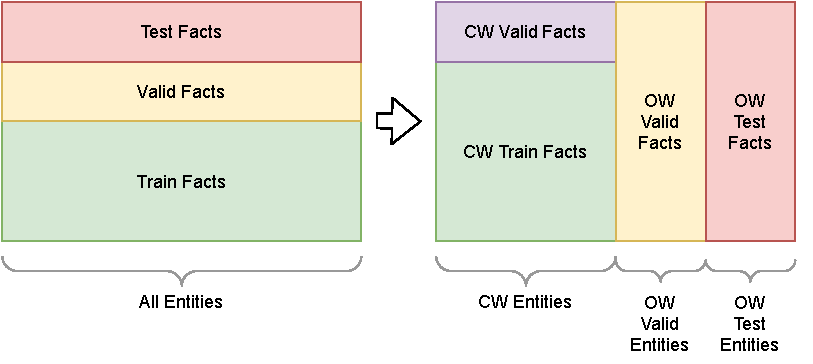
\includegraphics[width=\textwidth]{5_experiments/1_data_sources/1_knowledge_graphs/irt_split}
    \caption{Difference between a conventional and an IRT fact split. The IRT fact split focuses on open-world entities that must stay unseen during training. ``CW'' = ``closed-world'', ``OW'' = ``open-world''.}
    \label{fig:5_experiments/1_data_sources/1_knowledge_graphs/irt_split}
\end{figure}

\autoref{fig:5_experiments/1_data_sources/1_knowledge_graphs/irt_split} illustrates the different shape of an IRT fact split compared to a conventional one: The closed-world entities' facts are split into closed-world training and closed-world validation facts to enable closed-world prediction. Meanwhile, the open-world entities' facts are completely reserved for validation and training, respectively. Closed-world training and closed-world validation facts only refer to closed-world entities. On the other hand, one of an open-world validation fact's head or tail may also be a closed-world entity, and one of an open-world test fact's head or tail may be a closed-world entity or an open-world validation entity. \autoref{tab:5_experiments/1_data_sources/1_knowledge_graphs/irt_splits} gives an overview of the scales of the IRT splits' entity and fact subsets.

\begin{table}[h]
    \centering
    \input{5_experiments/1_data_sources/1_knowledge_graphs/irt_splits}
    \caption{Scale of the IRT splits of the FB15k-237 and CoDEx-M datasets}
    \label{tab:5_experiments/1_data_sources/1_knowledge_graphs/irt_splits}
\end{table}


\subsection{Text Sets}
\label{subsec:5_experiments/1_data_sources/2_text_sets}
In addition to the open-world fact splits of FB15k-237 and CoDEx-M, Hamann provides multiple text sets for each split's entities. Thereby, the text sets' contents vary in quality and quantity, ranging from text sets that offer single, very specific entity descriptions to text sets that provide multiple low-quality contexts not necessarily describing the entity directly. Some of the text sets contain plain text, some mark the entity's mentions within the text via special tokens, and some mask the entity mention. Together with the choice between FB15k-237 and CoDEx-M, this allows for graph-text combinations suiting different real-world scenarios.

Table~\ref{tab:5_experiments/1_data_sources/2_text_sets/text_sets_table} lists some example sentences from selected text sets and shortly describes the naming schema behind the text sets' names that will be used throughout this chapter, while Table~\ref{tab:a_appendix/text_sets_all} in Appendix~\ref{ch:a_appendix} lists all text sets. For example, the text set named "cde-irt-5-marked" indictates that it contains up to five marked sentences for each entity in the CoDEx-M graph. Thereby, the four dash-separated name parts denote (1) the graph for whose entities texts are provided, (2) the texts' origin, (3) the maximum number of sentences per entity and (4) whether the sentences are marked masked. There are three types of sentences that are distinguished by their source:

\begin{itemize}
    \item The \emph{CDE sentences} were provided by the authors of the CoDEx paper~\cite{}. They are the entities' first sentence from their respective Wikipedia page and thus very specific.
    \item The \emph{IRT sentences} have been introduced in Hamann's IRT paper~\cite{}. They are randomly sampled entity contexts from the English Wikipedia that mention the entity in a more or less meaningful way anywhere in the sentence.
    \item The \emph{OWE sentences} are very compact entity descriptions, often consisting of only a few words. They were created by Villmov et al. during the work on their OWE model for open-world KGC~\cite{Shah2019AnOE}.
\end{itemize}

\begin{table}
    \centering
    \input{5_experiments/1_data_sources/2_text_sets/text_sets_table}
    \caption{Example sentences from some of the text sets. The text set name a-b-c-d reveals (a) the graph ("fb" = FB15k-237, "cde" = CoDEx-M), (b) the text origin ("cde", "irt", "owe"), (c) the maximum number of sentences per entity and (d) whether entity mentions are marked or masked.}
    \label{tab:5_experiments/1_data_sources/2_text_sets/text_sets_table}
\end{table}




\section{Power Splits}
\label{sec:5_experiments/2_power_splits}
\begin{tabular}{| l | r | r | r | r | r |}
    \hline
    
    \multicolumn{1}{|c|}{\textbf{Power Split}} &
    \multicolumn{1}{|c|}{\textbf{\thead{Train Facts}}} &
    \multicolumn{1}{|c|}{\textbf{\thead{Known \\ Valid Facts}}} &
    \multicolumn{1}{|c|}{\textbf{\thead{Known \\ Valid Facts \\ per Entity}}} &
    \multicolumn{1}{|c|}{\textbf{\thead{Known \\ Test Facts}}} &
    \multicolumn{1}{|c|}{\textbf{\thead{Known \\ Test Facts \\ per Entity}}} \\

    \hline\hline

    CDE-0   & \multirow{6}{*}{\num{137738}} & \num{0}     & \num{0.00} & \num{0}     & \num{0.00} \\
    CDE-5   &                               & \num{2062}  & \num{0.71} & \num{1378}  & \num{0.73} \\
    CDE-15  &                               & \num{6186}  & \num{2.12} & \num{4136}  & \num{2.18} \\
    CDE-30  &                               & \num{12372} & \num{4.24} & \num{8273}  & \num{4.36} \\
    CDE-50  &                               & \num{20620} & \num{7.07} & \num{13788} & \num{7.27} \\
    CDE-100 &                               & \num{?}     & \num{7.07} & \num{13788} & \num{7.27} \\

    \hline

    FB-0   & \multirow{6}{*}{\num{238191}} & \num{0}     & \num{0.00}  & \num{0}     & \num{0.0} \\
    FB-5   &                               & \num{2325}  & \num{1.50}  & \num{1271}  & \num{1.56} \\
    FB-15  &                               & \num{6975}  & \num{4.51}  & \num{3813}  & \num{4.67} \\
    FB-30  &                               & \num{13950} & \num{9.03}  & \num{7626}  & \num{9.35} \\
    FB-50  &                               & \num{23251} & \num{15.05} & \num{12711} & \num{15.58} \\
    FB-100 &                               & \num{?}     & \num{15.05} & \num{12711} & \num{15.58} \\
    
    \hline
\end{tabular}



\section{Texter}
\label{sec:5_experiments/3_texter}
While the Ruler processes the query entity's known facts, the Texter takes the entity's sentences to predict facts. Although it can only predict the most common facts from the training set, its main advantage is its applicability to open-world entities that come without any known facts about them.

\subsection{Simple Model}
\label{subsec:4_approach/1_texter/1_simple_model}
During inference, the first step of processing a query entity, which is the same for both the simple and the attentive Texter, is embedding the entity's sentences in the embedding block. Thereby, each sentence is processed individually as illustrated in Figure~\ref{fig:4_approach/1_texter/1_simple_model/simple_architecture}: First, the sentence is split into words by the tokenizer, which are handled as integer IDs in further processing. Next, the words are embedded using some NLP approach, which could be a simple lookup table in the simplest case. As the last step in the embedding block, the word embeddings are combined to sentence embeddings in the pooling layer. The resulting sentence embeddings, that capture the sentences' overall meanings, are then passed on to the classification block where each of them is pushed through the neural multi-label classifier which consists of a single linear layer. Another pooling layer then combines the sentence-wise classification logits to the entity's logits. Finally, applying the sigmoid function to the entity's logits yields the class probabilites that state the probabilities of the associated facts about the query entity.

\begin{figure}[t]
    \centering
    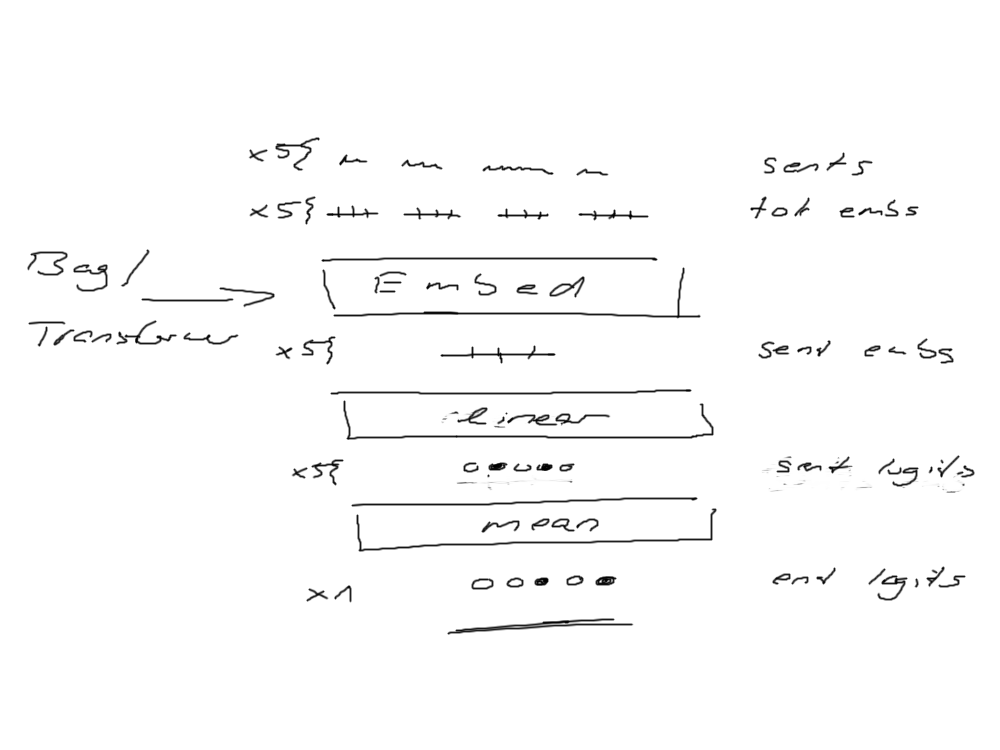
\includegraphics{4_approach/1_texter/1_simple_model/simple_architecture}
    \caption{Simple Texter Architecture; Each sentence is embedded and classified individually before the final pooling layer combines the results; "++++----" represents an embedding with positive and negative elements}
    \label{fig:4_approach/1_texter/1_simple_model/simple_architecture}
\end{figure}

Especially in the embedding block there are different possibilities for the concrete implementation of the individual parts to choose from, some of which will be examined in Chapter~\ref{ch:5_experiments}. In the final version of the power model, a transformer model is used for embedding the sentences' words, more precisely DistilBERT, a "distilled" variant of the transformer encoder BERT reduced to the essentials~\cite{Sanh2019DistilBERTAD}. In contrast to a simple lookup table, DistilBERT is able to incorporate the context of a word into its embedding, which leads to more meaningful sentence embeddings. This choice of embedding approach also affects the tokenizer, the pooling layer, and even the input sentences: Thanks to context embedding, transformers can use special tokens that add additional information to the text. While a classical model cannot decide on the basis of the sentence "Lisa likes John." whether this sentence speaks for the class $(x, has~gender, male)$, a transformer is able to do so given the appropriately marked sentence "Lisa likes [START]John[END].". Especially for long, ambigious sentences performance can be increased significantly.

Beyond the input data, the use of a transformer also affects the tokenizer and the pooling layer. The tokenizer has to apply byte pair encoding (BPE) that is commonly used by pre-trained transformers, where sentences are not only divided into words, but words are further divided into subwords, thus keeping the vocabulary of the tokenizer small and allowing to exploit homorphisms between similar words. In addition, the tokenizer inserts the [CLS] and [SEP] introduced by BERT at the beginning and end of the sentence. That way, "Lisa likes [START]John[END]." becomes "[CLS]Lisa likes [START]John[END].[SEP]". While the [SEP] token is used to separate sentences and has no further meaning here, the embedding of the [CLS] token captures the meaning of the whole sentence and is therefore  used as a sentence representation in the BERT paper~\cite{Devlin2019BERTPO}. However, the power experiments showed that performance can be increased if the word embeddings are also included, which is why the pooling layer of the embedding block averages all of a sentence's token embeddings, including the [CLS] embedding.

Less comprehensive processing steps happen in the classification block of the simple Texter: The sentence embeddings produced by the embedding block are pushed through the single linear classification layer whose multi-label output logits are averaged in the final pooling layer. The class probabilities calculated by applying the sigmoid function to the resulting entity logits are then used to sort the facts that have a probability greater than 50\%. Thus, the user of the model first receives the facts that are most likely to apply.


\subsection{Attention Model}
\label{subsec:4_approach/1_texter/2_attention_model}
While the simple Texter produces good evaluation results and does return a prioritized list of predicted facts, its prediction miss the desired explanation of why a fact is suggested. At this point, the attentive Texter extends the simple model by an attention mechanism that compares an entitiy's sentences to each other, forcing the model to favor sentences that are most relevant to the prediction of a certain fact. Besides the ability to provide an explanations for its predictions, the added attention mechanism should also increase the Texter's performance on datasets with multiple sentences per entity.

Technically, the attention mechanism is implemented as an attention block between the embedding and the classification blocks as shown in Figure~\ref{fig:4_approach/1_texter/2_attention_model/attention_architecture}. The embedding block is the same one used in the simple model, leveraging the DistilBERT encoder's contextual word embeddings to support marked input sentences and produce meaningful sentence embeddings. The classification block still produces the entity's multi-label output logits, but now uses multiple smaller linear layers to do so, due to the different outputs passed in from the attention block.

\begin{figure}[t]
    \centering
    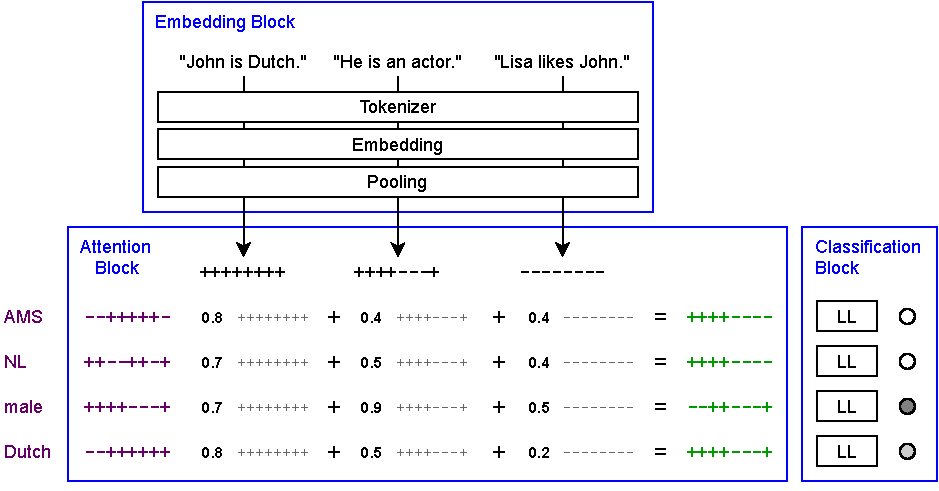
\includegraphics{4_approach/1_texter/2_attention_model/attention_architecture}
    \caption{Texter Architecture}
    \label{fig:4_approach/1_texter/2_attention_model/attention_architecture}
\end{figure}

The attention block now takes the sentence embeddings from the embedding block and compares them to so-called \emph{class embeddings} that represent each of the models output classes as a vector of the same dimension as the sentence embeddings. Given the set of input sentences $S$ and the set of classes $C$, the similarity between a class embedding $class_c$ and a sentence embedding $sent_s$ with $1 <= c <= |C|$ and $1 <= s <= |S|$ is calculated as the scalar product $\langle class_c, sent_s \rangle$ between the class and the sentece embedding. Given all class-sentence similarities for a certain class, the model can decide which sentence is matches the best for that class and deserves most attention when it comes to the decision whether the class holds true. Therefore, those similarity values are also referred to as attention values. To minimize the effect of sentences whose embeddings are very similar to a class embedding by pure chance, the attention values are furthermore normalized using the sigmoid function. Thus, the total attention matrix containing the attention values for all combinations of classes from $C$ and sentences from $S$ is calculated as shown in Equation~\ref{eq:4_approach/1_texter/2_attention_model/attention_matrix}.

\begin{align}
    A_{cs} = \sigma(\langle class_c , sent_s \rangle) && 1 <= c <= |C|, 1 <= s <= |S|
    \label{eq:4_approach/1_texter/2_attention_model/attention_matrix}
\end{align}

In the next step, the calculated attention values are used to combine the sentence embeddings to class-wise entity embeddings $ent_c$. As illstrated in Figure~\ref{fig:4_approach/1_texter/2_attention_model/attention_architecture} and formalized in Equation~\ref{eq:4_approach/1_texter/2_attention_model/ent_emb}, each sentence is thereby weighted by its class-wise attention value. The weighted sentences are then summed up to form class-wise entity embeddings whose purpose is to capture primarily those texts most relevant to the prediction of the respective class. Different from the simple Texter, the entity embeddings are then passed to the subsequent classification block instead of the original sentence embeddings.

\begin{align}
    ent_c = \sum_{s = 1}^{|S|} A_{cs} \cdot sent_s && 1 <= c <= |C|, 1 <= s <= |S|
    \label{eq:4_approach/1_texter/2_attention_model/ent_emb}
\end{align}

Similar to the simple Texter, the attentive Texter's classification consists of a $|C| \times d$ weight matrix and a bias vector of length $d$ where $d$ is the chosen embedding dimensionality for word, sentence, class and entity embeddings. In contrast to the simple model, however, given an entity embedding for a certain class, the weight matrix is not trained with respect to all output classes at once, but only with respect to the regarded class' ground truth output as illustrated in Figure~\ref{fig:4_approach/1_texter/2_attention_model/multi_linear}, which conceptually can be seen as training a separate single-output linear layer for each class and combining the outputs to the multi-label output thereafter. Formally, the models output classification outputs can be calculated as $out_c = \langle ent_c, W_c \rangle + b_c$ where $W_c$ and $b_c$ are the class' row in the weight matrix and its bias, respectively. The described approach to training the weight matrix was chosen, because a certain class' entity embedding focuses on the prediction of a single output class and would only hinder the learning process for other output classes it cannot make a qualified statement about.

\begin{figure}[t]
    \centering
    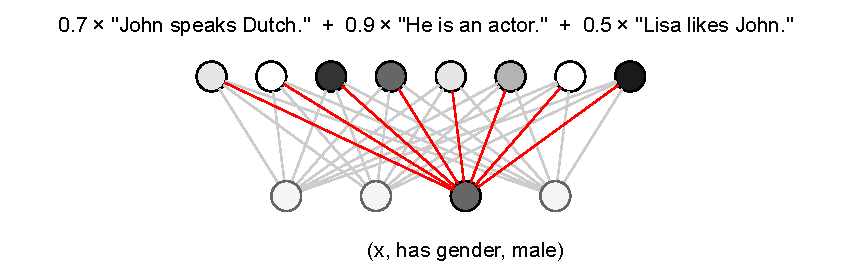
\includegraphics{4_approach/1_texter/2_attention_model/multi_linear}
    \caption{Multi-linear}
    \label{fig:4_approach/1_texter/2_attention_model/multi_linear}
\end{figure}

Similar to the simple Texter, following the core steps, the attentive Texter takes all classes whose confidences, that result from applying the sigmoid function to the output logits, is greater than 50\% to form their corresponding facts and sort them by confidence. In addition to the simple Texter, however, the attentive model provides the facts with the sentence weights as they result from the attention matrix in order to provide the user with an explanation for each fact's prediction. So, in the example, the fact $(John, has~gender, male)$, with a probability around 70\%, would be accompanied by the information that it was primarily suggested due to the sentence "He is an actor.", followed by "John speaks Dutch." and lastly "Lisa likes John.".

learnable class embs
sigmoid maps to (0, 1)
attention matrix A
total number of learnable params
in experiments: applied by an AdamW optimizer, a variant of the Adam optimizer that overcomes Adam's that keeps the training speed of Adam while keeping SGD's superior ability to generalize~, \cite{Loshchilov2019DecoupledWD}




\section{Ruler}
\label{sec:5_experiments/4_ruler}
While the Texter processes the text information attached to the knowledge graph's entities, the Ruler exploits patterns in the graph structure to predict missing facts. Given an entity $x$ with a set of known facts $K$ containing facts of the form $(x, rel_k, tail_k)$ with $1 <= k <= |K|$ and $rel_k \in R$ and $tail_k \in E$ being any relation or entity, respectively, the Ruler leverages entity-related rules of the form $(x, rel_m, tail_m) <= (x, rel_k, tail_k)$ with $1 <= m <= |M|$ to predict a set of missing facts $M$. Therefore, the rules required for the inference process have to be mined from the knowledge graph, beforehand. That rule mining process can be viewed as the equivalent to the Texter's training process and some paragraphs in this thesis will refer to combined rule mining and creation of a Ruler as "training" a Ruler. Compatibel to the Texter, the Ruler is limited to the prediction of facts $(x, rel, tail)$ that contain the query entity as their head, as well. However, when the Ruler is applied to all entities $e \in E$, all facts of the form $(e, rel, x)$ are predicted at some point as far as the mined rules support it.

For rule mining, AnyBURL, the bottom-up rule mining algorithm, by Christian Meilicke et al.~\cite{Meilicke2019AnytimeBR} is used. It is an anytime algorithm, meaning that it can be interrupted anytime and still yield valid results. Bottom-up rule mining refers to the fact that the algorithm starts with concrete paths in the graph and tries to generalize those paths to rules instead of coming up with rules initially and searching for evidence later, which would be a top-down approach. Out of all possible Horn rules that might describe patterns in the graph, AnyBURL is restricted to rules that can be generalized from so-called \emph{ground path rules}. A ground path rule does not contain variables, but only constants, and must not contain any cycles in its body. Equation~\ref{eq:4_approach/2_ruler/ground_path_rule} describes the general form of a ground path rule of length $n$, meaning that it consists out of the head fact and $n$ body facts.

\begin{align}
(c_0, h, c_1)
    \Leftarrow (c_1, b_1, c_2), \dots, (c_n, b_n, c_{n+1}) &&
    c_k \neq c_l \forall k, l \in \{1, \dots, n+1\}, k \ne l
    \label{eq:4_approach/2_ruler/ground_path_rule}
\end{align}

Notably, despite the rule body being free of cycles, the ground path rule as a whole can still be cyclic if $c_0 = c_{n+1}$. Ground path rules are derived directly from randomly sampled paths in the graph and are subsequently generalized to rules that replace some of the constants with variables. If further supporting paths can be found for a general rule, it is kept. In their paper on AnyBURL, Meilicke et al. show that any rule that can be generalized from a ground path rules can be generalized to one of the three rule types formulated in Equations~\ref{eq:4_approach/2_ruler/c}~--~\ref{eq:4_approach/2_ruler/ac2}. Thereby, $C$-type rules can only be generalized from cyclic ground path rules, $AC2$ rules can only be generalized from acyclic ground path rules and $AC1$ can be generalized from both, cyclic and acyclic ground path rules. The following paragraphs outline the core algorihm used to mine such rules and derive some example rules from the small graph introduced in Chapter~\ref{ch:1_introduction}. Figure~\ref{fig:4_approach/2_ruler/rule_graph} shows an annotated subset of the graph that illustrates the rules. "Amsterdam" and "Netherlands" have been abbreviated to "AMS" and "NL" to keep the examples short.

\begin{align}
    C   && (Y, h, X)   &\Leftarrow (X, b_1, A_2), \dots, (A_n, b_n, Y)
    \label{eq:4_approach/2_ruler/c} \\
    AC1 && (c_0, h, X) &\Leftarrow (X, b_1, A_2), \dots, (A_n, b_n, c_{n+1})
    \label{eq:4_approach/2_ruler/ac1} \\
    AC2 && (c_0, h, X) &\Leftarrow (X, b_1, A_2), \dots, (A_n, b_n, A_{n+1})
    \label{eq:4_approach/2_ruler/ac2}
\end{align}

\begin{figure}[t]
    \centering
    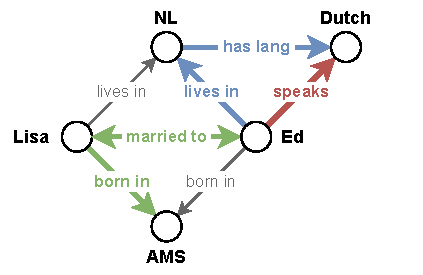
\includegraphics{4_approach/2_ruler/rule_graph}
    \caption{Subset of the previously introduced example graph with highlighted facts that form an acyclic (red + green) and a cyclic (red + blue) path.}
    \label{fig:4_approach/2_ruler/rule_graph}
\end{figure}

Essentially, AnyBURL repeatedly samples random paths from the graphs, generalizes them to all possible rule types, looks for further paths that match the gained rules, and keeps those rules it finds further evidence for. For example, in search of rules of length 2, i.e. rules that have a body consisting of 2 facts, AnyBURL might randomly sample the two paths in~\ref{eq:4_approach/2_ruler/path_1} and~\ref{eq:4_approach/2_ruler/path_2} from the graph. Note, that parentheses denote entities, brackets denote relations and that the path does not need to follow directed edges in the graph. Furthermore, a close look at the paths reveals that the second path is cyclic as it starts and ends at the entity "Dutch".

\begin{align}
(Dutch)
    \leftarrow [speaks] - (Ed) - [married~to] \rightarrow (Lisa) - [born~in] \rightarrow (AMS)
    \label{eq:4_approach/2_ruler/path_1} \\
    (Dutch) \leftarrow [speaks] - (Ed) - [lives~in] \rightarrow (NL) - [has~lang] \rightarrow (Dutch)
    \label{eq:4_approach/2_ruler/path_2}
\end{align}

From those paths, AnyBURL would then derive the constant-only
ground path rules~\ref{eq:4_approach/2_ruler/acyclic_ground_path} and~\ref{eq:4_approach/2_ruler/cyclic_ground_path} by taking the path's first part as the rule's head and the remaining parts to form the rule's body.

\begin{align}
(Ed, speaks, Dutch)
    &\Leftarrow (Ed, married~to, Lisa), (Lisa, born~in, AMS)
    \label{eq:4_approach/2_ruler/acyclic_ground_path} \\
    (Ed, speaks, Dutch) &\Leftarrow (Ed, lives~in, NL), (NL, has~lang, Dutch)
    \label{eq:4_approach/2_ruler/cyclic_ground_path}
\end{align}

The acyclic ground path rule in~\ref{eq:4_approach/2_ruler/acyclic_ground_path} can be generalized to the $AC1$ rule~\ref{eq:4_approach/2_ruler/acyclic_ac1} and the $AC2$ rule~\ref{eq:4_approach/2_ruler/acyclic_ac2} while the cyclic ground path rule~\ref{eq:4_approach/2_ruler/cyclic_ground_path} can be generalized to the $C$ rule~\ref{eq:4_approach/2_ruler/cyclic_c} and the $AC1$ rule~\ref{eq:4_approach/2_ruler/cyclic_ac1}.

\begin{align}
    AC1 && (X, speaks, Dutch) &\Leftarrow (X, married~to, A_2), (A_2, born~in, AMS)
    \label{eq:4_approach/2_ruler/acyclic_ac1} \\
    AC2 && (X, speaks, Dutch) &\Leftarrow (X, married~to, A_2), (A_2, born~in, A_3)
    \label{eq:4_approach/2_ruler/acyclic_ac2} \\
        C   && (X, speaks, Y) &\Leftarrow (X, lives~in, A_2), (A_2, has~lang, Y)
    \label{eq:4_approach/2_ruler/cyclic_c} \\
    AC1 && (X, speaks, Dutch) &\Leftarrow (X, lives~in, A_2), (A_2, has~lang, Dutch)
    \label{eq:4_approach/2_ruler/cyclic_ac1}
\end{align}

Next, every rule candidate is scored by looking for further paths that match the rule's body and checking whether the graph also contains the fact predicted by the rule, i.e. whether the rule is correct in that case. Thereby, the number of paths that match the rule body is called the rule's \emph{support} while the ratio of times the rule is correct over its total support is called \emph{confidence}. Taking the cyclic rule~\ref{eq:4_approach/2_ruler/cyclic_c} as an example, AnyBURL would search for further evidence and find the path $(Lisa) - [lives~in] -> (NL) - [has~lang] -> (Dutch)$ that matches the rule body, increasing the rule's support to two, so far. However, the example graph does not contain the rule's predicted fact $(Lisa, speaks, Dutch)$, so the rule's support drops from 1 to $\frac{1}{2}$. Since rules that only apply to a single case or only once in every thousands case are not very useful, AnyBURL drops rules with a support of 1 or confidence below 0.0001 by default~\cite{AnyBURL}. It is noteworthy that, although some rules are more general than others, such as~\ref{eq:4_approach/2_ruler/acyclic_ac2} compared to~\ref{eq:4_approach/2_ruler/acyclic_ac1}, the more specific ones are still kept as they might end up with higher confidence for their special case during the ongoing mining process.

The process described by the above example is repeated until only few new rules of the same length $n$ can be found. AnyBURL then continues its search for rules of length $n + 1$ until it terminates after a fixed number of time steps. Listing~\ref{code:anyburl} shows the slightly adjusted pseudocode from the AnyBURL paper. The sampling and scoring process discussed above is implemented as the body of the inner while loop. The outer for loop implements the repeated check for the saturation of rules of the current length and the eventual proceeding to rules of increased length.

% TODO param s

\begin{listing}[t]
    \begin{lstlisting}
        AnyBURL(G, sat, Q, i, ts):
            n = 2
            R = $\emptyset$
            for i times:
                $R_s = \emptyset$
                start = current_time()
                while current_time() < start + ts:
                    p = sample_path(G, n)
                    $R_p$ = generate_rules(p)
                    for $r$ in $R_p$:
                        score($r$)
                        if $Q$($r)$:
                            $R_s$ = $R_s \cup {r}$

                $R_s^{'}$ = $R_s \cap R$
                if $|R_s^{'}| / |R_s| > sat$:
                    n = n + 1
                $R$ = $R \cup R_s$

            return $R$
    \end{lstlisting}
    \caption{The AnyBURL rule mining algorithm takes a graph $G$, a saturation level $sat$, a quality criterion $Q$, and a number of iterations $i$, each of a timespan $ts$, as input and produces a ruleset $R$.}
    \label{code:anyburl}
\end{listing}

A walk through the pseudocode reads as follows: Given the Graph $G$, the saturation threshold $s$, the quality criterion $Q$, a number of iterations $i$ and the timespan $ts$ each iteration endures, AnyBURL starts with an empty ruleset $R$, that will be extended after each iteration and returned in the end. The initial length of the randomly sampled paths is $n=2$, allowing to find the shortest possible rules of length 1. During the first iteration of duration $ts$, AnyBURL fills the rule set $R_s$, that keeps the rules found in the current iteration, by repeatedly sampling paths, generating rules from the paths, scoring the resulting rules, and keeping those with sufficient support and confidence. At the end of the iteration, when the timespan $ts$ has passed, $R_s^{'}$ is calculated as the set of rules mined during the iteration that were already known. If the share of already known rules mined during the current iteration exceeds the saturation threshold, the algorithm starts searching for rules of increased length. Otherwise, it continues with the current length. In both cases, the iteration's rules are added to the overall ruleset $R$. If the specified number of total iterations is reached, AnyBURL terminates and returns the mined rules $R$. In practice, AnyBURL saves the mined rules in a text file at the end and at configurable points during mining.

With the stored rules from AnyBURL in place, the Ruler is prepared for inference. Conceptually, given an entity and its known facts, the Ruler loads the rules, filters out further rules that do not meet the Ruler's quality demands and applies the remaining, useful rules to all known facts. All rules that can be applied successfully are kept together with their confidence. From all the facts predicted by the applied rules, already known facts from the existing graph are filtered out. The remaining facts are sorted by confidence and returned to the user - together with the rules that predicted them as an explanation for the user. If multiple rules predict the same fact, the fact is assigned the highest confidence of those rules and is returned together with all of them. The Ruler's extra quality criterion mentioned above further restricts the considered rules to those with confidence greater 50\%, because AnyBURL's minimum confidence threshold of 0.01\% allows many rules that predict false positives. For open-world entities, this algorithm implies an empty result set as no rule can cover an entity that is not connected to any other entity and all the facts predicted for the train entities will be filtered out. In those cases, the Power model has to rely solely on the Texter.



\section{Aggregator}
\label{sec:5_experiments/5_aggregator}
The aggregator has the task of merging the predicted facts from Ruler and Texter. As envisioned in \autoref{sec:4_approach/3_aggregator} and illustrated in \autoref{fig:4_approach/3_aggregator/lucy}, it was hoped that merging the facts leads to higher average precision because facts predicted by both components are likely to be correct and should be ranked higher. In addition, the Aggregator should be able to estimate how reliable the predictions of Ruler and Texter are in relation to each other, which is implemented in the form of the weight parameter $\alpha$ as described in \autoref{eq:4_approach/3_aggregator/conf_aggregator}.

\autoref{tab:5_experiments/5_aggregator/results} shows the final evaluation results for the Aggregator, and thus the final evaluation results for the Power model, for a number of graph-text combinations. As fact splits, the splits with 50\% known test facts were chosen, as for the final Ruler evaluation in \autoref{sec:5_experiments/4_ruler}. The respective results for the CDE-50 and FB-50 splits from \autoref{tab:5_experiments/4_ruler/results} were taken over into \autoref{tab:5_experiments/5_aggregator/results} for easier comparability. Similarly, the chosen text sets are the ones from the final Texter evaluation in \autoref{subsec:5_experiments/3_texter/3_context}. Again, \autoref{tab:5_experiments/5_aggregator/results} duplicates the respective results from \autoref{tab:5_experiments/3_texter/3_context/results} for ease of comparison. The last two columns then contain the new Aggregator measurements for the combination of the corresponding Ruler and Texter.

\begin{table}[t]
    \makebox[\textwidth][c]{
        \begin{tabular}{ l l c r r r }
    \toprule

    \multicolumn{1}{l}{\textbf{Text Set}} &
    \multicolumn{1}{l}{\textbf{Texter}} & \phantom &
    \multicolumn{3}{c}{\textbf{Macro over Classes}} \\

    \cmidrule{4-6}

    & 
    &&
    \multicolumn{1}{c}{\textbf{Prec}} &
    \multicolumn{1}{c}{\textbf{Rec}} &
    \multicolumn{1}{c}{\textbf{F1}} \\
    
    \midrule

    \multirow{2}{*}{cde-cde-1-clean}
    & Simple    && \textbf{49.02} & 47.57 & 47.67 \\
    & Attentive && 46.86 & \textbf{51.09} & \textbf{47.98} \\

    \addlinespace

    \multirow{2}{*}{cde-irt-1-clean}
    & Simple    && 25.20 & \textbf{34.18} & \textbf{28.13} \\
    & Attentive && \textbf{26.70} & 31.41 & 27.43 \\

    \addlinespace

    \multirow{2}{*}{cde-irt-5-clean}
    & Simple    && 36.49 & \textbf{44.38} & \textbf{38.98} \\
    & Attentive && \textbf{39.20} & 37.11 & 36.98 \\

    \addlinespace

    \multirow{2}{*}{cde-irt-15-clean}
    & Simple    && 41.83 & \textbf{48.69} & \textbf{44.07} \\
    & Attentive && \textbf{44.63} & 37.39 & 39.78 \\

    \addlinespace

    \multirow{2}{*}{cde-irt-30-clean}
    & Simple    && 40.73 & \textbf{50.09} & \textbf{44.11} \\
    & Attentive && \textbf{43.60} & 36.10 & 38.78 \\
    
    \midrule

    \multirow{2}{*}{fb-owe-1-clean}
    & Simple    && 42.36 & \textbf{86.72} & 54.03 \\
    & Attentive && \textbf{45.21} & 84.03 & \textbf{56.16} \\

    \addlinespace

    \multirow{2}{*}{fb-irt-1-clean}
    & Simple    && 26.40 & 46.68 & 32.51 \\
    & Attentive && \textbf{27.01} & \textbf{49.90} & \textbf{34.26} \\

    \addlinespace

    \multirow{2}{*}{fb-irt-5-clean}
    & Simple    && 34.37 & \textbf{55.95} & 40.88 \\
    & Attentive && \textbf{39.21} & 50.63 & \textbf{43.50} \\

    \addlinespace

    \multirow{2}{*}{fb-irt-15-clean}
    & Simple    && \textbf{48.95} & \textbf{54.85} & \textbf{50.06} \\
    & Attentive && 48.89 & 52.75 & 49.92 \\

    \addlinespace

    \multirow{2}{*}{fb-irt-30-clean}
    & Simple    && 43.90 & \textbf{63.31} & \textbf{50.55} \\
    & Attentive && \textbf{50.57} & 48.47 & 48.79 \\
    
    \bottomrule
\end{tabular}

    }
    \caption{Final Aggregator results, i.e. final results for the Power model. The results of the Ruler and Texter, whose predictions the Aggregator combines, are also shown for comparison. Although the Aggregator does not outperform its respective Ruler and Texter in terms of F1 score, it does for mAP.}
    \label{tab:5_experiments/5_aggregator/results}
\end{table}

As the mAP values show, the Aggregator performs several percentage points better than the Ruler and Texter on their own, with the improvement on the CDE split being more obvious. However, the relatively small increase on the FB split suggests that the true positives of Ruler and Texter almost coincide there. For the CDE split, on the other hand, manually peeking into the predictions reveals that the improved mAP mainly results from complementary true positives -- and not so much from improved ranks of joint predictions. Looking at the values of simple and attentive Texter, it is also noticeable that the lead of the simple Texter over the attentive Texter shrinks when adding the Ruler. Likewise, the lead of the text sets with many sentences and with high-quality sentences shrinks. Finally, the different aptitudes for Ruler and Overall, the Aggregator results are even similar between the two splits, while previously, models performed significantly better on the FB split.

Two experiments that will be mentioned only briefly here, because of their unspectacular results, concerning the calculation of the Aggregator's confidence as per \autoref{eq:4_approach/3_aggregator/conf_aggregator}: First, in the beginning, experiments were conducted on the computation of the combined confidence $conf_{Aggregator}$ in cases where facts are predicted by Ruler and Texter. As combining methods, calculating the maximum and the mean of $conf_{Ruler}$ and $conf_{Texter}$ were evaluated, but it soon became apparent that summing them up much better accommodates the fact that a fact predicted by Ruler and Texter deserves very high confidence. Second, experiments showed that taking into account the weight parameter $\alpha$ between Ruler and Texter yields only marginal performance improvements in the tenths of a percent range because the confidence values of Ruler and Texter seem to be very comparable after all and thus always yield $\alpha$ values close to 0.5. In detail, Ruler and Texer were both a bit too optimistic about their predictions in the experiments -- but they were equally overconfident.




    \chapter{Conclusion}
    \label{ch:6_conclusion}
    Knowledge graphs are used in more and more domains and research on AI assisted knowledge graph completion enjoys increasing interest. Due to the ongoing exponential information growth~\cite{}, especially of freely accessible texts on the web~\cite{}, it is becoming easier to obtain additional entity information that can be used to improve the predictions of KGC models.

In this work, the Power ensemble model was developed which uses complementary rule-based and text-based components to determine new facts for a knowledge graph for whose entities textual descriptions are available. The rule-based component exploits patterns in the graph structure found by the rule miner AnyBURL while the text-based component uses the state-of-the-art transformer DistilBERT to effectively evaluate texts. Thanks to the rule-based component and an attention mechanism within the text-based component, the Power model also has the advantage over existing embedding-based models that it can provide human-understandable information about which rules and which texts were decisive for the predictions.

In a series of experiments, the model was evaluated on several combinations of graphs and text sets. Furthermore, different variations of the components were compared and the optimal conditions for training were determined. For the text-based component, this yielded the surprising finding that very good results can already be obtained without the use of computationally intensive transformers. Moreover, the attention mechanism was qualitatively tested for its functionality - and although the attention mechanism does not improve the performance, it nevertheless causes the comprehensible prioritization of the sentences. Overall, it was found that, depending on the graph and text inventory, sometimes the rule-based component and sometimes the text-based component provided better predictions, but the Power model as a whole always provided better results than either component on its own.

Building on the results of this thesis, future studies could address the following aspects in order to further improve the quality of the predicted facts:

\begin{itemize}
    \item The predicted facts could be used as a basis for the inference of further facts by repeatedly applying the known rules to the new facts. The predicted facts would be extended step by step until at some point they would correspond to the hull of all facts derivable from the given facts. Thereby, the probabilities of the underlying premises would have to be taken into account when calculating the probabilities of derived facts. With such an extension, transitive relations, such as ``is part of'' could be fully exploited and the rule-based component could participate in processing open-world entity which lack initially known facts.

    \item The model could be extended to include head prediction, i. e. given an entity $x$, predict facts of the form $(head, rel, x)$ without having to wait for the processing of the entity $head$.

    \item The rule-based component is currently limited to processing the particularly common, reliable AnyBURL rules of type $AC_1$ of length 1, and could be extended to rules of types $AC_2$ and $C$, as well as rules of arbitrary length.

    \item In terms of the ranking scenario, evaluation of rules with a confidence lower than 0.5 could be considered to achieve higher average precision. At the same time, new metrics like precision@k could be considered to check if the increased mAP is also reflected in the top predictions.

    \item It could be investigated whether splitting the classifier used in the text-based component into several smaller classifiers gives an advantage in regard to unbalanced classes.
\end{itemize}


    \newpage

    \bibliographystyle{plain}

    \begin{btSect}{main}
        \section*{References}
        \btPrintCited
    \end{btSect}

    \begin{btSect}{online}
        \section*{Online Sources}
        \btPrintCited
    \end{btSect}


    \appendix


    \chapter{Tables and Plots}
    \label{ch:a_appendix}
    \begin{table}
    \centering
    \begin{tabular}{| l | l |}
    \hline

    \multicolumn{1}{|c|}{\textbf{Text Set}} &
    \multicolumn{1}{|c|}{\textbf{Description}} \\

    \hline \hline

    cde-cde-1-clean   & One CDE sentence per CDE entity                \\

    \hline

    cde-irt-1-clean   & One IRT sentence per CDE entity                \\
    cde-irt-1-marked  & One marked IRT sentence per CDE entity         \\
    cde-irt-1-masked  & One masked IRT sentence per CDE entity         \\

    \hline

    cde-irt-5-clean   & Up to five CDE sentences per CDE entity        \\
    cde-irt-5-marked  & Up to five marked CDE sentences per CDE entity \\
    cde-irt-5-masked  & Up to five masked CDE sentences per CDE entity \\

    \hline

    cde-irt-15-clean  & Up to 15 CDE sentences per CDE entity          \\
    cde-irt-15-marked & Up to 15 marked CDE sentences per CDE entity   \\
    cde-irt-15-masked & Up to 15 masked CDE sentences per CDE entity   \\

    \hline

    cde-irt-30-clean  & Up to 30 CDE sentences per CDE entity          \\
    cde-irt-30-marked & Up to 30 marked CDE sentences per CDE entity   \\
    cde-irt-30-masked & Up to 30 masked CDE sentences per CDE entity   \\

    \hline \hline

    fb-irt-1-clean    & One IRT sentence per FB entity                 \\
    fb-irt-1-marked   & One marked IRT sentence per FB entity          \\
    fb-irt-1-masked   & One masked IRT sentence per FB entity          \\

    \hline

    fb-irt-5-clean    & Up to 5 IRT sentences per FB entity            \\
    fb-irt-5-marked   & Up to 5 marked IRT sentences per FB entity     \\
    fb-irt-5-masked   & Up to 5 masked IRT sentences per FB entity     \\

    \hline

    fb-irt-15-clean   & Up to 15 IRT sentences per FB entity           \\
    fb-irt-15-marked  & Up to 15 marked IRT sentences per FB entity    \\
    fb-irt-15-masked  & Up to 15 masked IRT sentences per FB entity    \\

    \hline

    fb-irt-30-clean   & Up to 30 IRT sentences per FB entity           \\
    fb-irt-30-marked  & Up to 30 marked IRT sentences per FB entity    \\
    fb-irt-30-masked  & Up to 30 masked IRT sentences per FB entity    \\

    \hline

    fb-owe-1-clean    & One OWE sentence per FB entity                 \\

    \hline
\end{tabular}

    \caption{List of the IRT~\cite{} text sets for the CoDEx-M (CDE) \cite{Safavi2020CoDExAC} and FB15k-237 (FB) \cite{Toutanova2015ObservedVL} entities used during evaluation}
    \label{tab:a_appendix/text_sets_all}
\end{table}

\begin{table}
    \centering
    \begin{tabular}{| l | r | r | r | r | r | r |}
    \hline

    \multicolumn{1}{|c|}{\textbf{Text Set}} &
    \multicolumn{3}{|c|}{\textbf{Simple Texter}}
    &
    \multicolumn{3}{|c|}{\textbf{Attending Texter}}
    \\

    \multicolumn{1}{|c|}{} &
    \multicolumn{1}{|c|}{\textbf{Prec}} &
    \multicolumn{1}{|c|}{\textbf{Rec}}
    &
    \multicolumn{1}{|c|}{\textbf{F1}}
    &
    \multicolumn{1}{|c|}{\textbf{Prec}}
    &
    \multicolumn{1}{|c|}{\textbf{Rec}}
    &
    \multicolumn{1}{|c|}{\textbf{F1}}
    \\

    \hline \hline

    cde-cde-1-clean   & 33.76 & 71.28 & 44.10 & 42.53 & 60.62 & 49.26 \\ \hline
    cde-irt-1-clean   & 24.66 & 56.31 & 32.83 & 28.07 & 41.03 & 32.80 \\
    cde-irt-1-marked  & 28.31 & 56.48 & 36.60 & 30.00 & 43.56 & 35.02 \\
    cde-irt-1-masked  & 25.30 & 52.19 & 32.98 & 27.64 & 35.08 & 30.49 \\ \hline
    cde-irt-5-clean   & 35.51 & 54.70 & 42.37 & 34.61 & 48.01 & 39.81 \\
    cde-irt-5-marked  & 37.63 & 52.25 & 43.26 & 37.12 & 49.56 & 41.88 \\
    cde-irt-5-masked  & 38.00 & 53.70 & 43.76 & 34.42 & 48.01 & 39.50 \\ \hline
    cde-irt-15-clean  & 40.13 & 54.34 & 45.22 & 39.88 & 47.16 & 42.80 \\
    cde-irt-15-marked & 37.89 & 55.32 & 44.50 & 39.14 & 51.96 & 44.04 \\
    cde-irt-15-masked & 43.26 & 54.55 & 47.37 & 38.90 & 50.39 & 43.39 \\ \hline
    cde-irt-30-clean  & 40.09 & 52.41 & 44.47 & 36.74 & 57.78 & 43.83 \\
    cde-irt-30-marked & 37.94 & 52.37 & 43.39 & 40.78 & 58.07 & 46.82 \\
    cde-irt-30-masked & 45.66 & 55.15 & 49.24 & 37.85 & 58.56 & 45.05 \\ \hline \hline
    fb-owe-1-clean    & 41.43 & 89.33 & 53.62 & 46.49 & 87.44 & 57.87 \\ \hline
    fb-irt-1-clean    & 33.18 & 61.56 & 40.19 & 33.76 & 52.08 & 39.56 \\
    fb-irt-1-marked   & 38.84 & 69.48 & 47.89 & 39.40 & 61.50 & 47.07 \\
    fb-irt-1-masked   & 33.28 & 69.95 & 43.07 & 35.36 & 58.49 & 43.11 \\ \hline
    fb-irt-5-clean    & 48.08 & 56.23 & 46.18 & 43.82 & 59.30 & 49.53 \\
    fb-irt-5-marked   & 46.91 & 64.77 & 53.16 & 45.84 & 71.21 & 54.28 \\
    fb-irt-5-masked   & 44.68 & 65.95 & 50.08 & 45.54 & 55.88 & 48.74 \\ \hline
    fb-irt-15-clean   & 49.07 & 58.46 & 49.69 & 49.72 & 69.46 & 56.93 \\
    fb-irt-15-marked  & 46.68 & 69.70 & 54.85 & 48.44 & 79.19 & 58.68 \\
    fb-irt-15-masked  & 44.39 & 79.43 & 53.74 & 47.79 & 71.52 & 56.34 \\ \hline
    fb-irt-30-clean   & 46.00 & 58.87 & 50.69 & 46.08 & 60.59 & 51.44 \\
    fb-irt-30-marked  & 45.50 & 61.38 & 51.10 & 52.54 & 64.47 & 56.78 \\
    fb-irt-30-masked  & 41.20 & 60.15 & 47.56 & 47.52 & 72.42 & 56.25 \\ \hline

\end{tabular}

    \caption{Context Final Precision Recall}
    \label{tab:a_appendix/context_final_prec_rec}
\end{table}

\begin{figure}[h]
    \centering
    \subfloat[cde-cde-1-simple]{
    \begin{tikzpicture}
    \begin{axis}[
        axis lines = middle,
        cycle list name = tb,
        grid = both,
        legend pos = outer north east,
        scale = 0.6,
        xlabel = epoch,
        ylabel = F1,
    ]
        \addplot table [x = Step, y = Value, col sep = comma] {a_appendix/static_classes_1/cde_cde_1_simple/class_1.csv};
        \addplot table [x = Step, y = Value, col sep = comma] {a_appendix/static_classes_1/cde_cde_1_simple/class_2.csv};
        \addplot table [x = Step, y = Value, col sep = comma] {a_appendix/static_classes_1/cde_cde_1_simple/class_3.csv};
        \addplot table [x = Step, y = Value, col sep = comma] {a_appendix/static_classes_1/cde_cde_1_simple/class_avg.csv};
        \addplot table [x = Step, y = Value, col sep = comma] {a_appendix/static_classes_1/cde_cde_1_simple/class_98.csv};
        \addplot table [x = Step, y = Value, col sep = comma] {a_appendix/static_classes_1/cde_cde_1_simple/class_99.csv};
        \addplot table [x = Step, y = Value, col sep = comma] {a_appendix/static_classes_1/cde_cde_1_simple/class_100.csv};
    \end{axis}
\end{tikzpicture}

    \label{fig:a_appendix/static_classes_1/cde_cde_1_simple}
}
\hskip 5pt
\subfloat[cde-cde-1-attentive]{
    \begin{tikzpicture}
    \begin{axis}[
        axis lines = middle,
        cycle list name = tb,
        grid = both,
        legend pos = outer north east,
        scale = 0.6,
        xlabel = epoch,
        ylabel = F1,
    ]
        \addplot table [x = Step, y = Value, col sep = comma] {a_appendix/static_classes_1/cde_cde_1_attentive/class_1.csv};
        \addplot table [x = Step, y = Value, col sep = comma] {a_appendix/static_classes_1/cde_cde_1_attentive/class_2.csv};
        \addplot table [x = Step, y = Value, col sep = comma] {a_appendix/static_classes_1/cde_cde_1_attentive/class_3.csv};
        \addplot table [x = Step, y = Value, col sep = comma] {a_appendix/static_classes_1/cde_cde_1_attentive/class_avg.csv};
        \addplot table [x = Step, y = Value, col sep = comma] {a_appendix/static_classes_1/cde_cde_1_attentive/class_98.csv};
        \addplot table [x = Step, y = Value, col sep = comma] {a_appendix/static_classes_1/cde_cde_1_attentive/class_99.csv};
        \addplot table [x = Step, y = Value, col sep = comma] {a_appendix/static_classes_1/cde_cde_1_attentive/class_100.csv};
    \end{axis}
\end{tikzpicture}

    \label{fig:a_appendix/static_classes_1/cde_cde_1_attentive}
}

\subfloat[cde-irt-1-simple]{
    \begin{tikzpicture}
    \begin{axis}[
        axis lines = middle,
        cycle list name = tb,
        grid = both,
        legend pos = outer north east,
        scale = 0.6,
        xlabel = epoch,
        ylabel = F1,
    ]
        \addplot table [x = Step, y = Value, col sep = comma] {a_appendix/static_classes_1/cde_irt_1_simple/class_1.csv};
        \addplot table [x = Step, y = Value, col sep = comma] {a_appendix/static_classes_1/cde_irt_1_simple/class_2.csv};
        \addplot table [x = Step, y = Value, col sep = comma] {a_appendix/static_classes_1/cde_irt_1_simple/class_3.csv};
        \addplot table [x = Step, y = Value, col sep = comma] {a_appendix/static_classes_1/cde_irt_1_simple/class_avg.csv};
        \addplot table [x = Step, y = Value, col sep = comma] {a_appendix/static_classes_1/cde_irt_1_simple/class_98.csv};
        \addplot table [x = Step, y = Value, col sep = comma] {a_appendix/static_classes_1/cde_irt_1_simple/class_99.csv};
        \addplot table [x = Step, y = Value, col sep = comma] {a_appendix/static_classes_1/cde_irt_1_simple/class_100.csv};
    \end{axis}
\end{tikzpicture}

    \label{fig:a_appendix/static_classes_1/cde_irt_1_simple}
}
\hskip 5pt
\subfloat[cde-irt-1-attentive]{
    \begin{tikzpicture}
    \begin{axis}[
        axis lines = middle,
        cycle list name = tb,
        grid = both,
        legend pos = outer north east,
        scale = 0.6,
        xlabel = epoch,
        ylabel = F1,
    ]
        \addplot table [x = Step, y = Value, col sep = comma] {a_appendix/static_classes_1/cde_irt_1_attentive/class_1.csv};
        \addplot table [x = Step, y = Value, col sep = comma] {a_appendix/static_classes_1/cde_irt_1_attentive/class_2.csv};
        \addplot table [x = Step, y = Value, col sep = comma] {a_appendix/static_classes_1/cde_irt_1_attentive/class_3.csv};
        \addplot table [x = Step, y = Value, col sep = comma] {a_appendix/static_classes_1/cde_irt_1_attentive/class_avg.csv};
        \addplot table [x = Step, y = Value, col sep = comma] {a_appendix/static_classes_1/cde_irt_1_attentive/class_98.csv};
        \addplot table [x = Step, y = Value, col sep = comma] {a_appendix/static_classes_1/cde_irt_1_attentive/class_99.csv};
        \addplot table [x = Step, y = Value, col sep = comma] {a_appendix/static_classes_1/cde_irt_1_attentive/class_100.csv};
    \end{axis}
\end{tikzpicture}

    \label{fig:a_appendix/static_classes_1/cde_irt_1_attentive}
}

\subfloat[cde-irt-5-simple]{
    \begin{tikzpicture}
    \begin{axis}[
        axis lines = middle,
        cycle list name = tb,
        grid = both,
        legend pos = outer north east,
        scale = 0.8,
        xlabel = epoch,
        ylabel = F1,
    ]
        \addplot table [x = Step, y = Value, col sep = comma] {plots/appendix/static_classes_all/cde_irt_5_simple/class_1.csv};
        \addplot table [x = Step, y = Value, col sep = comma] {plots/appendix/static_classes_all/cde_irt_5_simple/class_2.csv};
        \addplot table [x = Step, y = Value, col sep = comma] {plots/appendix/static_classes_all/cde_irt_5_simple/class_3.csv};
        \addplot table [x = Step, y = Value, col sep = comma] {plots/appendix/static_classes_all/cde_irt_5_simple/class_avg.csv};
        \addplot table [x = Step, y = Value, col sep = comma] {plots/appendix/static_classes_all/cde_irt_5_simple/class_98.csv};
        \addplot table [x = Step, y = Value, col sep = comma] {plots/appendix/static_classes_all/cde_irt_5_simple/class_99.csv};
        \addplot table [x = Step, y = Value, col sep = comma] {plots/appendix/static_classes_all/cde_irt_5_simple/class_100.csv};
    \end{axis}
\end{tikzpicture}

    \label{fig:a_appendix/static_classes_1/cde_irt_5_simple}
}
\hskip 5pt
\subfloat[cde-irt-5-attentive]{
    \begin{tikzpicture}
    \begin{axis}[
        axis lines = middle,
        cycle list name = tb,
        grid = both,
        legend pos = outer north east,
        scale = 0.6,
        xlabel = epoch,
        ylabel = F1,
    ]
        \addplot table [x = Step, y = Value, col sep = comma] {a_appendix/static_classes_1/cde_irt_5_attentive/class_1.csv};
        \addplot table [x = Step, y = Value, col sep = comma] {a_appendix/static_classes_1/cde_irt_5_attentive/class_2.csv};
        \addplot table [x = Step, y = Value, col sep = comma] {a_appendix/static_classes_1/cde_irt_5_attentive/class_3.csv};
        \addplot table [x = Step, y = Value, col sep = comma] {a_appendix/static_classes_1/cde_irt_5_attentive/class_avg.csv};
        \addplot table [x = Step, y = Value, col sep = comma] {a_appendix/static_classes_1/cde_irt_5_attentive/class_98.csv};
        \addplot table [x = Step, y = Value, col sep = comma] {a_appendix/static_classes_1/cde_irt_5_attentive/class_99.csv};
        \addplot table [x = Step, y = Value, col sep = comma] {a_appendix/static_classes_1/cde_irt_5_attentive/class_100.csv};
    \end{axis}
\end{tikzpicture}

    \label{fig:a_appendix/static_classes_1/cde_irt_5_attentive}
}

\subfloat[cde-irt-15-simple]{
    \begin{tikzpicture}
    \begin{axis}[
        axis lines = middle,
        cycle list name = tb,
        grid = both,
        legend pos = outer north east,
        scale = 0.6,
        xlabel = epoch,
        ylabel = F1,
    ]
        \addplot table [x = Step, y = Value, col sep = comma] {a_appendix/static_classes_1/cde_irt_15_simple/class_1.csv};
        \addplot table [x = Step, y = Value, col sep = comma] {a_appendix/static_classes_1/cde_irt_15_simple/class_2.csv};
        \addplot table [x = Step, y = Value, col sep = comma] {a_appendix/static_classes_1/cde_irt_15_simple/class_3.csv};
        \addplot table [x = Step, y = Value, col sep = comma] {a_appendix/static_classes_1/cde_irt_15_simple/class_avg.csv};
        \addplot table [x = Step, y = Value, col sep = comma] {a_appendix/static_classes_1/cde_irt_15_simple/class_98.csv};
        \addplot table [x = Step, y = Value, col sep = comma] {a_appendix/static_classes_1/cde_irt_15_simple/class_99.csv};
        \addplot table [x = Step, y = Value, col sep = comma] {a_appendix/static_classes_1/cde_irt_15_simple/class_100.csv};
    \end{axis}
\end{tikzpicture}

    \label{fig:a_appendix/static_classes_1/cde_irt_15_simple}
}
\hskip 5pt
\subfloat[cde-irt-15-attentive]{
    \begin{tikzpicture}
    \begin{axis}[
        axis lines = middle,
        cycle list name = tb,
        grid = both,
        legend pos = outer north east,
        scale = 0.6,
        xlabel = epoch,
        ylabel = F1,
    ]
        \addplot table [x = Step, y = Value, col sep = comma] {a_appendix/static_classes_1/cde_irt_15_attentive/class_1.csv};
        \addplot table [x = Step, y = Value, col sep = comma] {a_appendix/static_classes_1/cde_irt_15_attentive/class_2.csv};
        \addplot table [x = Step, y = Value, col sep = comma] {a_appendix/static_classes_1/cde_irt_15_attentive/class_3.csv};
        \addplot table [x = Step, y = Value, col sep = comma] {a_appendix/static_classes_1/cde_irt_15_attentive/class_avg.csv};
        \addplot table [x = Step, y = Value, col sep = comma] {a_appendix/static_classes_1/cde_irt_15_attentive/class_98.csv};
        \addplot table [x = Step, y = Value, col sep = comma] {a_appendix/static_classes_1/cde_irt_15_attentive/class_99.csv};
        \addplot table [x = Step, y = Value, col sep = comma] {a_appendix/static_classes_1/cde_irt_15_attentive/class_100.csv};
    \end{axis}
\end{tikzpicture}

    \label{fig:a_appendix/static_classes_1/cde_irt_15_attentive}
}

    \caption{Development of the F1 score on the validation data during training}
    \label{fig:a_appendix/static_classes_1}
\end{figure}

\begin{figure}[h]
    \centering
    \subfloat[cde-irt-30-simple]{
    \begin{tikzpicture}
    \begin{axis}[
        axis lines = middle,
        cycle list name = tb,
        grid = both,
        legend pos = outer north east,
        scale = 0.6,
        xlabel = epoch,
        ylabel = F1,
    ]
        \addplot table [x = Step, y = Value, col sep = comma] {a_appendix/static_classes_2/cde_irt_30_simple/class_1.csv};
        \addplot table [x = Step, y = Value, col sep = comma] {a_appendix/static_classes_2/cde_irt_30_simple/class_2.csv};
        \addplot table [x = Step, y = Value, col sep = comma] {a_appendix/static_classes_2/cde_irt_30_simple/class_3.csv};
        \addplot table [x = Step, y = Value, col sep = comma] {a_appendix/static_classes_2/cde_irt_30_simple/class_avg.csv};
        \addplot table [x = Step, y = Value, col sep = comma] {a_appendix/static_classes_2/cde_irt_30_simple/class_98.csv};
        \addplot table [x = Step, y = Value, col sep = comma] {a_appendix/static_classes_2/cde_irt_30_simple/class_99.csv};
        \addplot table [x = Step, y = Value, col sep = comma] {a_appendix/static_classes_2/cde_irt_30_simple/class_100.csv};
    \end{axis}
\end{tikzpicture}

    \label{fig:a_appendix/static_classes_2/cde_irt_30_simple}
}
\hskip 5pt
\subfloat[cde-irt-30-attentive]{
    \begin{tikzpicture}
    \begin{axis}[
        axis lines = middle,
        cycle list name = tb,
        grid = both,
        legend pos = outer north east,
        scale = 0.6,
        xlabel = epoch,
        ylabel = F1,
    ]
        \addplot table [x = Step, y = Value, col sep = comma] {a_appendix/static_classes_2/cde_irt_30_attentive/class_1.csv};
        \addplot table [x = Step, y = Value, col sep = comma] {a_appendix/static_classes_2/cde_irt_30_attentive/class_2.csv};
        \addplot table [x = Step, y = Value, col sep = comma] {a_appendix/static_classes_2/cde_irt_30_attentive/class_3.csv};
        \addplot table [x = Step, y = Value, col sep = comma] {a_appendix/static_classes_2/cde_irt_30_attentive/class_avg.csv};
        \addplot table [x = Step, y = Value, col sep = comma] {a_appendix/static_classes_2/cde_irt_30_attentive/class_98.csv};
        \addplot table [x = Step, y = Value, col sep = comma] {a_appendix/static_classes_2/cde_irt_30_attentive/class_99.csv};
        \addplot table [x = Step, y = Value, col sep = comma] {a_appendix/static_classes_2/cde_irt_30_attentive/class_100.csv};
    \end{axis}
\end{tikzpicture}

    \label{fig:a_appendix/static_classes_2/cde_irt_30_attentive}
}

\subfloat[fb-irt-1-simple]{
    \begin{tikzpicture}
    \begin{axis}[
        axis lines = middle,
        cycle list name = tb,
        grid = both,
        legend pos = outer north east,
        scale = 0.6,
        xlabel = epoch,
        ylabel = F1,
    ]
        \addplot table [x = Step, y = Value, col sep = comma] {a_appendix/static_classes_2/fb_irt_1_simple/class_1.csv};
        \addplot table [x = Step, y = Value, col sep = comma] {a_appendix/static_classes_2/fb_irt_1_simple/class_2.csv};
        \addplot table [x = Step, y = Value, col sep = comma] {a_appendix/static_classes_2/fb_irt_1_simple/class_3.csv};
        \addplot table [x = Step, y = Value, col sep = comma] {a_appendix/static_classes_2/fb_irt_1_simple/class_avg.csv};
        \addplot table [x = Step, y = Value, col sep = comma] {a_appendix/static_classes_2/fb_irt_1_simple/class_98.csv};
        \addplot table [x = Step, y = Value, col sep = comma] {a_appendix/static_classes_2/fb_irt_1_simple/class_99.csv};
        \addplot table [x = Step, y = Value, col sep = comma] {a_appendix/static_classes_2/fb_irt_1_simple/class_100.csv};
    \end{axis}
\end{tikzpicture}

    \label{fig:a_appendix/static_classes_2/fb_irt_1_simple}
}
\hskip 5pt
\subfloat[fb-irt-1-attentive]{
    \begin{tikzpicture}
    \begin{axis}[
        axis lines = middle,
        cycle list name = tb,
        grid = both,
        legend pos = outer north east,
        scale = 0.6,
        xlabel = epoch,
        ylabel = F1,
    ]
        \addplot table [x = Step, y = Value, col sep = comma] {a_appendix/static_classes_2/fb_irt_1_attentive/class_1.csv};
        \addplot table [x = Step, y = Value, col sep = comma] {a_appendix/static_classes_2/fb_irt_1_attentive/class_2.csv};
        \addplot table [x = Step, y = Value, col sep = comma] {a_appendix/static_classes_2/fb_irt_1_attentive/class_3.csv};
        \addplot table [x = Step, y = Value, col sep = comma] {a_appendix/static_classes_2/fb_irt_1_attentive/class_avg.csv};
        \addplot table [x = Step, y = Value, col sep = comma] {a_appendix/static_classes_2/fb_irt_1_attentive/class_98.csv};
        \addplot table [x = Step, y = Value, col sep = comma] {a_appendix/static_classes_2/fb_irt_1_attentive/class_99.csv};
        \addplot table [x = Step, y = Value, col sep = comma] {a_appendix/static_classes_2/fb_irt_1_attentive/class_100.csv};
    \end{axis}
\end{tikzpicture}

    \label{fig:a_appendix/static_classes_2/fb_irt_1_attentive}
}

\subfloat[fb-irt-5-simple]{
    \begin{tikzpicture}
    \begin{axis}[
        axis lines = middle,
        cycle list name = tb,
        grid = both,
        legend pos = outer north east,
        scale = 0.6,
        xlabel = epoch,
        ylabel = F1,
    ]
        \addplot table [x = Step, y = Value, col sep = comma] {a_appendix/static_classes_2/fb_irt_5_simple/class_1.csv};
        \addplot table [x = Step, y = Value, col sep = comma] {a_appendix/static_classes_2/fb_irt_5_simple/class_2.csv};
        \addplot table [x = Step, y = Value, col sep = comma] {a_appendix/static_classes_2/fb_irt_5_simple/class_3.csv};
        \addplot table [x = Step, y = Value, col sep = comma] {a_appendix/static_classes_2/fb_irt_5_simple/class_avg.csv};
        \addplot table [x = Step, y = Value, col sep = comma] {a_appendix/static_classes_2/fb_irt_5_simple/class_98.csv};
        \addplot table [x = Step, y = Value, col sep = comma] {a_appendix/static_classes_2/fb_irt_5_simple/class_99.csv};
        \addplot table [x = Step, y = Value, col sep = comma] {a_appendix/static_classes_2/fb_irt_5_simple/class_100.csv};
    \end{axis}
\end{tikzpicture}

    \label{fig:a_appendix/static_classes_2/fb_irt_5_simple}
}
\hskip 5pt
\subfloat[fb-irt-5-attentive]{
    \begin{tikzpicture}
    \begin{axis}[
        axis lines = middle,
        cycle list name = tb,
        grid = both,
        legend pos = outer north east,
        scale = 0.6,
        xlabel = epoch,
        ylabel = F1,
    ]
        \addplot table [x = Step, y = Value, col sep = comma] {a_appendix/static_classes_2/fb_irt_5_attentive/class_1.csv};
        \addplot table [x = Step, y = Value, col sep = comma] {a_appendix/static_classes_2/fb_irt_5_attentive/class_2.csv};
        \addplot table [x = Step, y = Value, col sep = comma] {a_appendix/static_classes_2/fb_irt_5_attentive/class_3.csv};
        \addplot table [x = Step, y = Value, col sep = comma] {a_appendix/static_classes_2/fb_irt_5_attentive/class_avg.csv};
        \addplot table [x = Step, y = Value, col sep = comma] {a_appendix/static_classes_2/fb_irt_5_attentive/class_98.csv};
        \addplot table [x = Step, y = Value, col sep = comma] {a_appendix/static_classes_2/fb_irt_5_attentive/class_99.csv};
        \addplot table [x = Step, y = Value, col sep = comma] {a_appendix/static_classes_2/fb_irt_5_attentive/class_100.csv};
    \end{axis}
\end{tikzpicture}

    \label{fig:a_appendix/static_classes_2/fb_irt_5_attentive}
}

\subfloat[fb-irt-15-simple]{
    \begin{tikzpicture}
    \begin{axis}[
        axis lines = middle,
        cycle list name = tb,
        grid = both,
        legend pos = outer north east,
        scale = 0.6,
        xlabel = epoch,
        ylabel = F1,
    ]
        \addplot table [x = Step, y = Value, col sep = comma] {a_appendix/static_classes_2/fb_irt_15_simple/class_1.csv};
        \addplot table [x = Step, y = Value, col sep = comma] {a_appendix/static_classes_2/fb_irt_15_simple/class_2.csv};
        \addplot table [x = Step, y = Value, col sep = comma] {a_appendix/static_classes_2/fb_irt_15_simple/class_3.csv};
        \addplot table [x = Step, y = Value, col sep = comma] {a_appendix/static_classes_2/fb_irt_15_simple/class_avg.csv};
        \addplot table [x = Step, y = Value, col sep = comma] {a_appendix/static_classes_2/fb_irt_15_simple/class_98.csv};
        \addplot table [x = Step, y = Value, col sep = comma] {a_appendix/static_classes_2/fb_irt_15_simple/class_99.csv};
        \addplot table [x = Step, y = Value, col sep = comma] {a_appendix/static_classes_2/fb_irt_15_simple/class_100.csv};
    \end{axis}
\end{tikzpicture}

    \label{fig:a_appendix/static_classes_2/fb_irt_15_simple}
}
\hskip 5pt
\subfloat[fb-irt-15-attentive]{
    \begin{tikzpicture}
    \begin{axis}[
        axis lines = middle,
        cycle list name = tb,
        grid = both,
        legend pos = outer north east,
        scale = 0.6,
        xlabel = epoch,
        ylabel = F1,
    ]
        \addplot table [x = Step, y = Value, col sep = comma] {a_appendix/static_classes_2/fb_irt_15_attentive/class_1.csv};
        \addplot table [x = Step, y = Value, col sep = comma] {a_appendix/static_classes_2/fb_irt_15_attentive/class_2.csv};
        \addplot table [x = Step, y = Value, col sep = comma] {a_appendix/static_classes_2/fb_irt_15_attentive/class_3.csv};
        \addplot table [x = Step, y = Value, col sep = comma] {a_appendix/static_classes_2/fb_irt_15_attentive/class_avg.csv};
        \addplot table [x = Step, y = Value, col sep = comma] {a_appendix/static_classes_2/fb_irt_15_attentive/class_98.csv};
        \addplot table [x = Step, y = Value, col sep = comma] {a_appendix/static_classes_2/fb_irt_15_attentive/class_99.csv};
        \addplot table [x = Step, y = Value, col sep = comma] {a_appendix/static_classes_2/fb_irt_15_attentive/class_100.csv};
    \end{axis}
\end{tikzpicture}

    \label{fig:a_appendix/static_classes_2/fb_irt_15_attentive}
}

    \caption{Development of the F1 score on the validation data during training}
    \label{fig:a_appendix/static_classes_2}
\end{figure}

\begin{figure}[h]
    \centering
    \subfloat[fb-irt-30-simple]{
    \begin{tikzpicture}
    \begin{axis}[
        axis lines = middle,
        cycle list name = tb,
        grid = both,
        legend pos = outer north east,
        scale = 0.6,
        xlabel = epoch,
        ylabel = F1,
    ]
        \addplot table [x = Step, y = Value, col sep = comma] {a_appendix/static_classes_3/fb_irt_30_simple/class_1.csv};
        \addplot table [x = Step, y = Value, col sep = comma] {a_appendix/static_classes_3/fb_irt_30_simple/class_2.csv};
        \addplot table [x = Step, y = Value, col sep = comma] {a_appendix/static_classes_3/fb_irt_30_simple/class_3.csv};
        \addplot table [x = Step, y = Value, col sep = comma] {a_appendix/static_classes_3/fb_irt_30_simple/class_avg.csv};
        \addplot table [x = Step, y = Value, col sep = comma] {a_appendix/static_classes_3/fb_irt_30_simple/class_98.csv};
        \addplot table [x = Step, y = Value, col sep = comma] {a_appendix/static_classes_3/fb_irt_30_simple/class_99.csv};
        \addplot table [x = Step, y = Value, col sep = comma] {a_appendix/static_classes_3/fb_irt_30_simple/class_100.csv};
    \end{axis}
\end{tikzpicture}

    \label{fig:a_appendix/static_classes_3/fb_irt_30_simple}
}
\hskip 5pt
\subfloat[fb-irt-30-attentive]{
    \begin{tikzpicture}
    \begin{axis}[
        axis lines = middle,
        cycle list name = tb,
        grid = both,
        legend pos = outer north east,
        scale = 0.6,
        xlabel = epoch,
        ylabel = F1,
    ]
        \addplot table [x = Step, y = Value, col sep = comma] {a_appendix/static_classes_3/fb_irt_30_attentive/class_1.csv};
        \addplot table [x = Step, y = Value, col sep = comma] {a_appendix/static_classes_3/fb_irt_30_attentive/class_2.csv};
        \addplot table [x = Step, y = Value, col sep = comma] {a_appendix/static_classes_3/fb_irt_30_attentive/class_3.csv};
        \addplot table [x = Step, y = Value, col sep = comma] {a_appendix/static_classes_3/fb_irt_30_attentive/class_avg.csv};
        \addplot table [x = Step, y = Value, col sep = comma] {a_appendix/static_classes_3/fb_irt_30_attentive/class_98.csv};
        \addplot table [x = Step, y = Value, col sep = comma] {a_appendix/static_classes_3/fb_irt_30_attentive/class_99.csv};
        \addplot table [x = Step, y = Value, col sep = comma] {a_appendix/static_classes_3/fb_irt_30_attentive/class_100.csv};
    \end{axis}
\end{tikzpicture}

    \label{fig:a_appendix/static_classes_3/fb_irt_30_attentive}
}

\subfloat[fb-owe-1-simple]{
    \begin{tikzpicture}
    \begin{axis}[
        axis lines = middle,
        cycle list name = tb,
        grid = both,
        legend pos = outer north east,
        scale = 0.6,
        xlabel = epoch,
        ylabel = F1,
    ]
        \addplot table [x = Step, y = Value, col sep = comma] {a_appendix/static_classes_3/fb_owe_1_simple/class_1.csv};
        \addplot table [x = Step, y = Value, col sep = comma] {a_appendix/static_classes_3/fb_owe_1_simple/class_2.csv};
        \addplot table [x = Step, y = Value, col sep = comma] {a_appendix/static_classes_3/fb_owe_1_simple/class_3.csv};
        \addplot table [x = Step, y = Value, col sep = comma] {a_appendix/static_classes_3/fb_owe_1_simple/class_avg.csv};
        \addplot table [x = Step, y = Value, col sep = comma] {a_appendix/static_classes_3/fb_owe_1_simple/class_98.csv};
        \addplot table [x = Step, y = Value, col sep = comma] {a_appendix/static_classes_3/fb_owe_1_simple/class_99.csv};
        \addplot table [x = Step, y = Value, col sep = comma] {a_appendix/static_classes_3/fb_owe_1_simple/class_100.csv};
    \end{axis}
\end{tikzpicture}

    \label{fig:a_appendix/static_classes_3/fb_owe_1_simple}
}
\hskip 5pt
\subfloat[fb-owe-1-attentive]{
    \begin{tikzpicture}
    \begin{axis}[
        axis lines = middle,
        cycle list name = tb,
        grid = both,
        legend pos = outer north east,
        scale = 0.6,
        xlabel = epoch,
        ylabel = F1,
    ]
        \addplot table [x = Step, y = Value, col sep = comma] {a_appendix/static_classes_3/fb_owe_1_attentive/class_1.csv};
        \addplot table [x = Step, y = Value, col sep = comma] {a_appendix/static_classes_3/fb_owe_1_attentive/class_2.csv};
        \addplot table [x = Step, y = Value, col sep = comma] {a_appendix/static_classes_3/fb_owe_1_attentive/class_3.csv};
        \addplot table [x = Step, y = Value, col sep = comma] {a_appendix/static_classes_3/fb_owe_1_attentive/class_avg.csv};
        \addplot table [x = Step, y = Value, col sep = comma] {a_appendix/static_classes_3/fb_owe_1_attentive/class_98.csv};
        \addplot table [x = Step, y = Value, col sep = comma] {a_appendix/static_classes_3/fb_owe_1_attentive/class_99.csv};
        \addplot table [x = Step, y = Value, col sep = comma] {a_appendix/static_classes_3/fb_owe_1_attentive/class_100.csv};
    \end{axis}
\end{tikzpicture}

    \label{fig:a_appendix/static_classes_3/fb_owe_1_attentive}
}

    \caption{Development of the F1 score on the validation data during training}
    \label{fig:a_appendix/static_classes_3}
\end{figure}


\end{document}
